%!TEX program = Traditional Builder with XeLaTeX
% 使ctexbook按单面打印模式排版
\documentclass[
  a4paper,
  zihao=-4,
  fontset=mac,
  AutoFakeBold,
  AutoFakeSlant,
  oneside]{ctexbook} 

% math
\usepackage{amsmath, amsthm, amssymb} % Math
\usepackage{wasysym} % Greek alphabets
\usepackage{unicode-math} % Greek alphabets, 替换原先的MnSymbol. NOTE: 但unicode-math只能在xelatex或者lualatex中使用
\usepackage{mathrsfs, amsfonts} % Math fonts

% document
\usepackage{geometry} % Formatting
\usepackage{graphicx} % Required for inserting images
\usepackage{titlesec} % 定制章节标题样式
\usepackage{titletoc} % 定制目录格式
\usepackage{fancyhdr} % 引入fancyhdr宏包来控制页眉页脚
\usepackage{caption} % 定义caption
\usepackage{etoolbox} % 脚注通篇连续编号
\usepackage{listings} % 代码输入
\usepackage{hologo} % LaTeX logo支持
\usepackage{setspace} % 占位

% citation
\usepackage{hyperref} % 引用链接
\usepackage[
  backend=biber,
  style=gb7714-2005,
  citestyle=authoryear,
  sorting=nyvt,
  maxnames=1,
  minnames=1,
  maxbibnames=99,
  doi=false,
  gbpub=false]{biblatex}

% table
\usepackage{xcolor} % color
\usepackage{booktabs} % 使用booktabs表格形式
\usepackage{tabularx} % 在表格中制造换行
\usepackage{array} % 行间距

% font
\usepackage{fontspec, xeCJK} % 控制字体
\usepackage{anyfontsize} % 控制字体大小和行距

% ---------------------- 设置页面边距 ---------------------- 
\geometry{
  a4paper,
  top=3.5cm, 
  bottom=2.5cm, 
  left=2.5cm, 
  right=2.5cm,
  headheight=2.5cm,
  footskip=2cm,
  bindingoffset=0cm
  }
\setlength{\oddsidemargin}{0pt} % 奇数页左边距偏移
\setlength{\evensidemargin}{0pt} % 偶数页左边距偏移

% ----------------------  标题与段落 ---------------------- 
% 设置中文模板的日期格式和摘要名称
\ctexset{
  today=big, % 日期格式为大写
  abstractname=简介 % 摘要名称设置为“简介”
}

% 设置chapter标题格式
\titleformat{\chapter}[block]
{\centering\zihao{3}\heiti} % 居中、三号、黑体
{\thechapter}
{1em}
{}
[\vspace{1ex}] % 段后空1行

% 设置chapter标题的前后间距
\titlespacing{\chapter}
{0pt} % 左边距
{1ex} % 段前空1行  
{1ex} % 段后空1行

% 重新定义section标题格式
\titleformat{\section}[hang]  % hang表示标题采用悬挂式样式
{\heiti\zihao{4}\raggedright}  % 黑体、四号、左对齐
{\thesection}{1em}{}  % 编号与标题间距1em

% 设置section标题的前后间距
\titlespacing{\section}
{0pt}  % 左边距
{1ex}  % 段前空1行
{1ex}  % 段后空1行

% 重新定义subsection标题格式
\titleformat{\subsection}[hang]  % hang表示标题采用悬挂式样式
{\heiti\zihao{-4}\raggedright}  % 黑体、小四号、左对齐
{\thesubsection}{1em}{}  % 编号与标题间距1em

% 设置subsection标题的前后间距
\titlespacing{\subsection}
{0pt}  % 左边距
{1ex}  % 段前空1行
{1ex}  % 段后空1行

% ----------------------  页眉、页码、脚注、锁进、行距 ---------------------- 
% 脚注通篇连续编号
\counterwithout{footnote}{chapter} 

% 修改脚注行距
\let\oldfootnote\footnote
\renewcommand{\footnote}[1]{%
  \oldfootnote{\setstretch{1.5}#1}% 设置脚注行距为 1.2 倍
}

% 添加首行缩进,两个字符
\usepackage{indentfirst}
\setlength{\parindent}{2em}

% 设置行距
\renewcommand{\baselinestretch}{1.0}
\setlength{\parskip}{0pt}
\linespread{1.5}  % 固定行距20磅约等于1.5倍行距

% 设置页眉样式
\pagestyle{fancy}
\fancyhf{} % 清空默认页眉页脚
\fancyhead[C]{\zihao{5} 浙江财经大学硕士毕业论文} % 设置字号与居中
\fancyfoot[C]{\thepage} % 居中显示页码

% ----------------------  设置字体 ---------------------- 
% 从本地创建字体命令
%\newfontfamily\mysongti[Path=./]{stsong.ttf}
%\newfontfamily\mykaiti[Path=./]{stkaiti.ttf}
%\newfontfamily\mykaitigb[Path=./]{kaiti_GB2312.ttf}
%\newfontfamily\myheiti[Path=./]{simhei.ttf}
%\newfontfamily\myxihei[Path=./]{stxihei.ttf}

\setCJKmainfont{简宋} % 设置默认中文字体为宋体
\setmainfont{Times New Roman} % 设置默认英文字体为Times New Roman
%\newfontfamily\kaiti{Kai}
\newfontfamily\kaitigb[Path=./]{楷体_GB2312.ttf}

% ------------------------ caption样式 ------------------------------
% 设置 caption 与 figure 之间的距离
\setlength{\abovecaptionskip}{11pt}
\setlength{\belowcaptionskip}{9pt}

% 设置表格的 caption 与 table 之间的垂直距离
\captionsetup[table]{skip=2pt}

% 设置图片的 caption 格式
\renewcommand{\thefigure}{\thechapter-\arabic{figure}}
\captionsetup[figure]{font=small,labelsep=space}

% 设置表格的 caption 格式
\renewcommand{\thetable}{\thechapter-\arabic{table}}
\captionsetup[table]{font=small,labelsep=space}

% ----------------------  宏包设置 ---------------------- 
% hyperref设置
\hypersetup{
  pdflang = zh-CN, % 设置PDF文档语言为简体中文
  pdftitle = {浙江财经大学学位论文-李晨逸}, % PDF标题
  pdfauthor = {Suicidal Bumblebee} % 作者
}%

% array调整表格行间距
\renewcommand{\arraystretch}{1.5}

% citation
\ExecuteBibliographyOptions{sortlocale=zh__pinyin} % 设置排序语言环境为中文拼音
\addbibresource{Papers.bib} % 添加文献bib文件
\DeclareSourcemap{
  \maps[datatype=bibtex]{
    \map{
      \step[fieldset=url, null] % 删除 url 字段
    }
    \map{
      \step[fieldset=librarycatalog, null] % 删除 librarycatalog 字段
    }
}}

% ---------------------- 基本信息 ----------------------

% maketitle information
\title{基于个人动态最优居住地选择视角的劳动力回流行为考察}
\author{Suicidal Bumblebee}
\date{Jan 2025}

% 中文题目
\newcommand{\thesisTitle}{基于个人动态最优居住地选择视角的劳动力回流行为考察}
% 英文题目
\newcommand{\thesisTitleEN}{A Study of Return Migration Behavior Based on Dynamic Optimal
Residential Location Decisions}

% cover information
\newcommand{\deptName}{经济学院}
\newcommand{\majorName}{西方经济学}
\newcommand{\yourName}{李晨逸}
\newcommand{\yourStudentID}{230507031002}
\newcommand{\mentorName}{吴意云}
\newcommand{\Today}{2025年4月}

% underline
\newcommand\dunderline[3][-1pt]{{%
  \setbox0=\hbox{#3}
  \ooalign{\copy0\cr\rule[\dimexpr#1-#2\relax]{\wd0}{#2}}}}

% -------------------- ToC setting --------------------



% -------------------- 文章内容 --------------------
\begin{document}

% ---------------------------------------- 封面 ----------------------------------------
% 简易自动生成标题封面
% \maketitle

% 自定义标题封面
\begin{titlepage}
\vspace*{-20mm}

\centering


\includegraphics[width=3cm]{images/logo/schoolLogo.png}\\

\includegraphics[width=5cm, height=1cm]{images/logo/schoolName.png}

\vspace*{10mm}

\begin{center}
{
\fontsize{26pt}{28pt}
\spaceskip=0.12em
\xspaceskip=0.12em
\textbf{
  %\songti
  {
    硕\hspace{5mm}士\hspace{5mm}研\hspace{5mm}究\hspace{5mm}生\hspace{5mm}毕\hspace{5mm}业\hspace{5mm}论\hspace{5mm}文
    }
  }
}

\vspace{20mm}

{
\fontsize{18pt}{20pt}
\textmd{
    \heiti{题目:}\thesisTitle
  }
}

\vspace{5mm}
\vspace{30mm}

\flushleft


\begin{spacing}{2}
{
  \hspace{27mm}
  %\mysongti
  \fontsize{16pt}{18pt}
  \selectfont{学生姓名:\dunderline[-10pt]{1pt}{\makebox[78mm][c]{\yourName}}}
}

{ 
  \hspace{27mm}
  %\mysongti
  \fontsize{16pt}{18pt}
  \selectfont{学\hspace{11mm}号:\dunderline[-10pt]{1pt}{\makebox[78mm][c]{\yourStudentID}}}
}

{
  \hspace{27mm}
  %\mysongti
  \fontsize{16pt}{18pt}
  \selectfont{指导教师:\dunderline[-10pt]{1pt}{\makebox[78mm][c]{\mentorName}}}
} 

{
  \hspace{27mm}
  %\mysongti
  \fontsize{16pt}{18pt}
  \selectfont{所在学院:\dunderline[-10pt]{1pt}{\makebox[78mm][c]{\deptName}}}
}

{
  \hspace{27mm}
  %\mysongti
  \fontsize{16pt}{18pt}
  \selectfont{专业名称:\dunderline[-10pt]{1pt}{\makebox[78mm][c]{\majorName}}}
}

\end{spacing}
\end{center}
\end{titlepage}

\frontmatter

% ---------------------------------------- 原创性声明 ----------------------------------------
%% 原创性声明页
% 无特殊要求,不用修改

\fancypagestyle{originality}{
  % 页眉高度
  \setlength{\headheight}{10pt}

  % 页眉和页脚(页码)的格式设定
  \fancyhf{}
  \fancyhead[]{}

  % 页眉分割线稍微粗一些
  \renewcommand{\headrulewidth}{0pt}
}

\pagestyle{originality}
% \topskip=0pt

% % 圆形数字编号定义
% \newcommand{\circled}[2][]{\tikz[baseline=(char.base)]
%   {\node[shape = circle, draw, inner sep = 1pt]
%   (char) {\phantom{\ifblank{#1}{#2}{#1}}};
%   \node at (char.center) {\makebox[0pt][c]{#2}};}}
% \robustify{\circled}

% 设置行间距
\setlength{\parskip}{0.4em}
\renewcommand{\baselinestretch}{1.41}

% 顶部空白
\vspace*{-6mm}

% 原创性声明部分
\begin{center}
  \heiti\zihao{2}\textmd{声明及论文使用的授权}
\end{center}

\vspace{10mm}


% 本部分字号为小三
\zihao{-3}

本人郑重声明所呈交的论文是我个人在导师的指导下独立完成的。除了文中特别加以标注和致谢的地方外,论文中不包含其他人已经发表或撰写的研究成果。

\vspace{15mm}

\begin{flushright}
  论文作者签名:\hspace{75mm}年\hspace{8mm}月\hspace{8mm}日
\end{flushright}

\vspace{40mm}

% 使用授权声明部分

\zihao{-3}

本人同意浙江财经大学有关保留使用学位论文的规定,即:学校有权保留送交论文的复印件,允许论文被查阅和借阅;学校可以上网公布全部内容,可以采用影印、缩印或其他复制手段保存论文。

\vspace*{15mm}

\begin{flushright}
  论文作者签名:\hspace{75mm}年\hspace{8mm}月\hspace{8mm}日
\end{flushright}

\newpage


% ---------------------------------------- 摘要 ----------------------------------------
\chapter{摘要}

\begin{center}
    {
    \zihao{3}基于个人动态最优居住地选择视角的劳动力回流行为考察
    }
\end{center}


{\zihao{-4}
{\heiti 摘要:}{\kaitigb 随着经济的发展与社会工业化带来的社会关系剧变,劳动力迁移形成有规律的迁移模式是必然的。不同于我国研究中的传统城乡二元对立语境,本文基于理性预期构造了动态最优住址选择模型,基于CFPS数据对2010年至2022年间我国各省的人口流动进行实证检验,并得到的结论是(xxx、xxx、xxx)。本文的贡献在于(xxx、xxx、xxx)。}

{\heiti 关键词:}{\kaitigb 动态迁移决策模型、劳动力迁移、收入引致、迁移摩擦}
}

% ---------------------------------------- Abstract ----------------------------------------
\chapter{Abstract}

\begin{center}
    {
    \zihao{4}
    \textbf{A Study of Return Migration Behavior Based on Dynamic Optimal Residential Location Decisions}
    }
\end{center}

{\zihao{-4}
\textbf{Abstract}: Here is the english version of abstract

\textbf{keywords}: a,b,c
}



\frontmatter
\renewcommand{\thepage}{\Roman{page}} % 将frontmatter页码改为大写罗马数字

% ---------------------------------------- 目录 ----------------------------------------
% 目录自动生成
%% 论文目录
% 没有特殊需要不用修改

%目录开始

% 调整目录行间距
\renewcommand{\baselinestretch}{1.35}
% 目录
\tableofcontents
\newpage


\newpage
\tableofcontents
\thispagestyle{empty}

\mainmatter
% ---------------------------------------- 绪论 ----------------------------------------
\newpage
% \setcounter{page}{1} % 页码从此处开始记录
\chapter{引言}

% 点明人口流动的不均匀
纵观古今内外,“人往高处走,水往低处流”的规律总是屡试皆准。早在上世纪末,以\textcite{krugmanIncreasingReturnsEconomic1991}和\textcite{fujitaSpatialEconomyCities1999}为代表的新经济地理学就指出经济活动的集中会产生规模经济和网络效应,促成产业集聚。经济的聚集会导致区域不平衡发展,人们倾向于从“边缘”地区流向产业集聚、薪资较高和就业机会多的“中心”地区,形成吸引效应,这使得劳动力迁移有了移动的规律。欧美国家作为世界上人均GDP最高的区域,吸引大量来自其他相对落后国家的居民。根据世界银行(World Bank Group)和美国移民委员会(American Immigration Councile)公布的数据,
2023年美国的人均GDP为82769美元,外来人口达到了4780万,移民占美国人口的 14.3\%,比 1970 年的 4.7\% 增长了约三倍。这一由经济集聚驱动的中心-边缘迁移模式,在全球范围内得到印证,而在快速城市化的中国,其表现尤为深刻和复杂。改革开放以来,随着现代化交通工具的普及和人口流动政策的放宽,劳动力自由流动在我国成为可能。解放的经济活力逐渐形成了“东富西穷、南富北穷”的局面。经济发展的不平衡不仅表现在地区收入差距上,也体现在人口分布的变化中。富裕地区吸引了大量来自相对贫困地区的劳动力。国家统计局2020年发布的《第七次人口普查》显示,流动人口达到3.76亿,占全国总人口比重分别为34.90\%和26.62\%,较2010年分别上涨88.52\%和69.72\%。
广东跨省流入高达2962.21万人,浙江也达到1618.65万人,上海跨省流入人口为1047.97万人。这三地的跨省流入人口数量位居前三。此外,北京流入841.8万人,位居第五。
同时,我国也存在多个人口输出大省\footnote{该数据来源于2010年的《第六次人口普查》。},例如
安徽省净向外输出约911万人,占本省户籍人口的13.29\%;
四川省净向外输出约956 万人,占本省户籍人口的10.63\%;
河南省净向外输出约约565万人,约占本省户籍人口的7\%。

% 介绍流动规律
在我国激烈的劳动力迁移浪潮中大致存在以下规律。
首先,劳动力净流入的区域符合常识中的迁移规律,劳动力从农村流向城市是迁移的主流趋势。大城市由于更高的工资水平、更丰富的就业资源、更高质量的基础服务设施,具有强大的虹吸效应,这一点与新经济地理学学者提出的观点相吻合。在可以预见的未来,这种劳动力向经济发达地区集中的趋势仍将持续。
其次,永久迁移与暂时性迁移之间存在显著差异。第七次人口普查显示,2020年时我国人户分离人口已达4.93亿,占总人口的34.16\%。(xxx)
并且,尽管总体上劳动力向发达地区流动,仍有部分劳动力回流到欠发达地区。这种反直觉的现象已被部分学者注意到(\textcite{ShiZhiLeiJiaTingBingFuJiaTingJueCeYuNongCunQianYiLaoDongLiHuiLiu2012},\textcite{RenYuanNongCunWaiChuLaoDongLiHuiLiuQianYiDeYingXiangYinSuHeHuiLiuXiaoYing2017}),表明某些群体在外迁后因各种原因选择返回原居住地,这揭示了迁移决策背后更为复杂的动机。\textcite{davanzoRepeatMigrationUnited1983}就指出过劳动力个体迁移行为的“反复无常”规律————尽管大多数个体从未迁徙,但迁徙的个体很可能会再次迁徙,通常会返回原籍地。这意味着迁徙决策应该被看作是一系列地点选择,个体知道有机会修改或逆转那些效果不佳的迁徙。

% 我国学术界对于劳动力研究存在不足
对于劳动力流动现象的研究,我国学术界长期围绕城乡二元分析框架与空间均衡模型展开。作为典型的发展中经济体,我国自计划经济时期形成的城乡二元结构构成了劳动力迁移的制度基础。改革开放后,工业化进程产生的劳动要素需求与农村剩余劳动力释放一拍即合,这一过程在学术研究领域直接映射为对传统二元经济理论的引用。其中,在\textcite{lewisEconomicDevelopmentUnlimited1954}二元对立模型基础上,
\textcite{todaroModelLaborMigration1969}通过引入失业率与预期收入,突破了无限劳动供给假设的刚性约束,其"即使存在失业风险,人口仍会因预期收入差距迁移"的核心命题,恰与中国城市化进程中农民工"候鸟式迁移"的特征契合,成为解释中国农民工流动现象的核心理论工具。而后,\textcite{harrisMigrationUnemploymentDevelopment1970}进一步将城市正规部门与非正规部门纳入分析框架,通过工资刚性与就业概率的动态调整机制,构建起解释发展中国家城市失业与农村劳动力持续涌入并存现象的理论模型。这种强调制度分割与部门差异的分析视角,为中国学者解析户籍制度、土地制度等特殊约束条件下的劳动力流动提供了重要切入点。如\textcite{XiongCaiYunNongMinGongChengShiDingJuZhuanYiJueCeYinSuDeTuiLaMoXingJiShiZhengFenXi2007}构建的农民工定居决策模型,通过引入城市拉力(就业机会、公共服务)与农村推力(土地保障弱化、收入差距)的交互作用,拓展了传统二元模型的解释维度。\textcite{HuangZhongHuaNongCunTuDiZhiDuAnPaiShiFouZuAiNongMinGongShiMinHuaTuoDaLuoMoXingTuoZhanHeYiWuShiShiZhengFenXi2014}通过嵌入土地保险功能变量,\textcite{ZhongShuiYingXiangChengRenKouLiuDongDeLiLunJieShiNongCunRenKouTuiChuShiJiaoTuoDaLuoMoXingDeZaiXiuZheng2015}纳入制度变迁因素。
部分文献虽然淡化了城乡之间的对立,但依然在均衡状态下分析工资和租金的确定,同时考虑移民流动对这些结果的影响。
\textcite{ZongJiaFengDaChengShiZhiFuLiaoGengGaoDeGongZiMa2015}构建的三部门Rosen-Roback模型揭示,中国大城市存在显著工资溢价且技能异质性导致差异化集聚收益:高技能劳动力通过知识溢出获取短期增长红利,而低技能群体则需经历长期调整方能获益。
\textcite{WangLiLiWoGuoRenKouQianYiChengBenChengShiGuiMoYuShengChanLu2020,WangLiLiTuDiGongGeiFangJieYuLaoDongLiKongJianPeiZhiXiaoLu2023,WangLiLiLaoDongLiLiuDongDuiChengShiGongZiYuFuLiDeYingXiangJiYuKongJianJunHengMoXingDeFenXi2024}通过将土地供给管制、迁移壁垒等制度变量内生化,定量识别出行政干预对劳动力空间配置的扭曲效应:建设用地指标的区域错配加剧东部大城市住房供给弹性不足,推高生活成本并阻碍生产率导向的人口集聚,导致2010年经济总产出损失达3\%-4\%。刘华仁(2024)则构建包含人力资本溢出效应的量化空间均衡模型,证明高技能劳动力的区域再配置可通过生产率与公共服务双重渠道提升社会福利,这为人才政策优化提供了理论依据。

% 逐渐引出动态方法
尽管现有研究取得显著进展,但传统劳动力迁移研究的局限性却愈发明显。首先,动态视角的缺位限制了理论的解释力。主流文献多依赖静态或比较静态分析,将迁移决策简化为单期最优选择,忽视了个体在生命周期内因人力资本积累、预期调整和制度环境变迁而产生的动态交互。例如,
\textcite{HanQiHengNongCunLaoDongLiQianYiMoCaYingXiangNongMinGongShuLiangYuGongZiJieGouMa2018}虽尝试通过OLG模型捕捉迁移行为的代际动态,但其模型仍未能内生化制度约束与技能积累的交互效应。其次,微观基础的薄弱削弱了研究的政策适用性。许多研究基于宏观数据分析迁移的总体趋势,未能深入探讨个体异质性因素(如风险偏好、社会网络或数字技能)对迁移路径分化的影响,导致模型缺乏行为依据,难以支持精准的政策仿真。最后,理论范式的滞后使得现有模型难以适应劳动力流动的新特征。随着城-城流动规模扩大和远程就业的兴起,传统城乡二元对立的分析框架无法解释迁移的可逆性、多向性和地理重构效应。这些局限使得学界难以回答两个核心问题:在面临户籍限制带来的未来不确定性与地区间显著的收入差距时,不同人力资本水平的个体是如何动态地权衡其迁移、定居或回流的决策路径的?制度变迁如何通过重塑迁移的成本-收益结构影响个体的跨期决策?

针对上述问题,本研究提出从静态均衡向动态演化、从宏观相关性向微观行为基础、从单向城乡迁移向多维空间重构的理论转向。为此,本文构建了一个动态离散选择模型,将劳动力回流建模为一个马尔可夫决策过程(Markov Decision Process, MDP)。与静态模型将迁移视为一次性选择不同,MDP框架将迁移刻画为一个关于信息和预期的序列学习与适应过程,这更符合劳动力在真实世界中“走一步看一步”的决策本质。该模型假设个体在有限生命周期内基于效用最大化原则选择居住地,效用函数综合考虑了地区吸引力(如工资和公共服务)、制度摩擦(如户籍限制)以及个体异质性(如乡土黏性和人力资本水平)。通过非参数混合估计方法,本研究量化以下机制:(1)户籍制度改革和土地确权如何通过提升预期稳定性增强迁移的持久性;(2)人力资本积累速率的差异如何导致迁移路径的分化,例如高技能个体更倾向于城市间的多次迁移;(3)远程就业的普及如何通过降低物理迁移成本重塑迁移的地理指向和频率。模型不仅为解析中国劳动力流动的复杂性提供了新的分析 工具,还通过揭示迁移决策的微观驱动因素,为优化区域发展和以人为核心的城镇化政策提供了实证依据。

% 本文重要性、创新性等
本文的重要性在于,在当前工业化加速和经济转型的背景下,劳动力跨区域迁移问题愈发显得关键而复杂。人口流动不仅直接影响城市化进程、区域经济平衡和资源配置效率,还对社会福利和经济结构的长期调整产生深远影响。尤其在中国这一快速发展的经济体中,劳动力回流现象既是城市化进程的缩影,也是城乡协调发展的关键变量。深入理解和准确预测劳动力迁移趋势,不仅有助于把握经济发展的内在动力,还为政策制定提供了科学依据,以实现区域协调发展和社会整体进步。

本研究从动态决策的视角切入,系统分析劳动力回流的规律及其驱动机制,特别强调收入差异作为核心经济因素的作用。与此同时,模型综合考虑了就业机会、生活成本、制度摩擦和文化因素的交互效应。例如,户籍制度作为中国特有的制度约束,可能通过限制公共服务获取提高迁移成本,从而影响个体是否选择永久定居城市。同样,地区间的文化差异(如方言)可能通过乡土黏性影响迁移决策的稳定性。通过构建理论模型并结合实证分析,本文旨在回答以下问题:地区间的收入差异如何激发劳动力迁移?收入差异如何与其他因素(如公共服务供给和户籍限制)共同作用于迁移决策?通过何种政策干预可以引导劳动力合理流动,从而优化资源配置、促进城乡协调发展并提升社会福利?

正如\textcite{desmetUrbanAccountingWelfare2013}在城市规模与福利分析中所指出的,理解决定人口分布的各种力量对于回答一系列关键问题至关重要:这些力量在决定城市规模分布中的相对重要性如何?如果各地区在公共服务、技术水平或制度摩擦方面趋于一致,人口将如何重新配置?这种重新配置对社会福利的总体影响是什么?这一论述启发本研究将收入差异置于更广泛的动态框架中,探讨其如何通过影响迁移决策重塑人口分布和区域经济格局。如果地区间的制度和经济差异缩小,劳动力流动和城市规模分布可能发生显著变化,进而影响整体社会福利。本研究通过量化这些机制,为劳动力迁移的理论和实证分析提供了一个综合框架。

% 结构安排
为实现上述研究目标,本文结构安排如下:第二章对国内外相关文献进行系统综述,梳理劳动力迁移的理论演进和实证成果,分析现有研究的不足,并明确本文的创新点。第三章构建动态离散选择模型,详细阐述模型的基本假设、机制设计以及与现实经济现象的关联,推导劳动力迁移存在性的理论命题。第四章推导实证分析所需的似然函数,说明模型简化的必要假设(如支撑点离散化处理未知分布),并介绍数据来源(中国家庭追踪调查和地区年鉴)、变量构造和Python实现的计算方法。第五章展示实证分析的主要结论,通过对不同样本子集的检验和命题验证,评估模型在解释中国劳动力回流中的适用性和稳健性。第六章总结研究的主要发现,讨论模型的局限性(如理性人假设的适用性、函数形式的潜在任意性),并提出未来研究方向,例如引入收入分配结构或跨省迁移的网络分析。
此外,更为详细的数学证明、高性能程序代码和数据处理流程均附在文末的附录中。

% ---------------------------------------- 文献综述 ----------------------------------------
\chapter{文献综述}

劳动力流动作为经济社会发展的重要表征,其研究要点在于提供合适的方法和寻找符合现实逻辑的影响因素。本文通过系统梳理国内外近几十年来的经典文献与前沿成果,试图厘清学术脉络的演进逻辑,为后续实证研究提供标准。
在研究方法层面,现有文献呈现出从静态分析向动态追踪的范式转变。就影响因素而言,学者们已逐步突破传统经济变量的单一解释,将制度约束、社会网络、文化认同等非经济维度纳入分析体系。


\section{相关概念梳理}
劳动力回流是指原先从一个地区迁出的劳动力再次返回原籍地的现象。这种迁移可被视为可撤回的(retractable)或短暂的(temporary),与传统静态迁移模型所假设的单向永久性迁移存在显著差异。

劳动力回流研究具有以下特点:首先,从历史维度看,它是一个相对较新的现象,在人类工业化历程中出现较晚;其次,它挑战了传统人口迁移理论中从欠发达地区向发达地区单向流动的基本假设;再次,对于后发工业化国家而言,这一现象具有重要的政策意义。

在传统经济理论框架下,当目标地经济衰退导致预期收益低于原籍地时,返迁决策符合理性选择理论;然而当目标地仍能提供显著收入溢价时,劳动力选择返迁则构成理论悖论。这一现象值得深入研究,特别是对于后发工业化国家而言。

\textcite{CaiFangHuJiZhiDuYuLaoDongLiShiChangBaoHu2001}等学者指出,后发国家通常采取非均衡发展战略,通过制度化的城乡二元结构形成工农产品价格剪刀差,实现资源从传统农业部门向现代工业部门的系统性转移。这种情况下,劳动力回流可能不利于资本深化与工业化进程。
中国的工业化路径具有特殊性,融合了社会主义国家计划经济与市场经济转型的特点。20世纪50至80年代,由于资源稀缺,我国建立了以户籍制度为核心的空间资源配置体系,将有限资本集中于少数城市,形成公共服务的高度集聚。改革开放后,我国借鉴东亚发展型国家经验,采取出口导向型发展战略,特别是2001年加入世贸组织后,充分发挥人口红利的比较优势。\textcite{LinYiFuZhongGuoDeJingJiFaZhanZhanLueYuDiQuShouRuChaiJu2003}为这一发展路径提供了系统的理论支撑。
在快速工业化进程中,大量人口涌入城市,形成了沿海发达地区持续吸纳内陆剩余劳动力的迁移格局。然而,我国劳动力市场中却出现明显的回流现象,即农村居民进城打工后又返回原籍,形成农民工返潮现象。这一现象与后发国家工业化进程中的劳动力配置目标存在理论上的背离。

多项研究表明,户籍制度障碍可能是影响劳动力定居的首要因素。\textcite{RenYuanChengShiLiuDongRenKouDeSheHuiRongHeWenXianShuPing2006}指出,以户籍制度为依托的流动人口管理制度及相关社会福利制度对流动人口的限制与排斥对其社会融合有根本性影响。\textcite{LuYiLongHuKouHuanQiZuoYongMaHuJiZhiDuYuSheHuiFenCengHeLiuDong2008}认为即使经历了深刻改革,户籍制度仍然对劳动力自由流动造成客观阻碍,制约经济高质量发展。
另一种观点认为,源于1994年分税制改革的土地财政模式可能是劳动力回流的重要原因。\textcite{ChenYingFangNongMinGongZhiDuAnPaiYuShenFenRenTong2005}、\textcite{niehuihuaZhongguogaofangjiadexinzhengzhijingjixuejieshiYiZhengqihemou2013}及\textcite{YuJianXingDiFangFaZhanXingZhengFuDeXingWeiLuoJiJiZhiDuJiChu2012}等研究认为,土地出让金作为地方政府重要财源,导致政府维持较高地价,推高房价,增加城市居民住房负担,从而影响劳动力的定居决策。

除户籍与土地财政外,影响劳动力回流的因素还可能包括原籍地经济发展与就业机会增加、工资差距缩小、生活成本差异变化;家庭纽带与社会融入因素;以及公共服务可及性、返乡创业政策等制度因素。
综合来看,劳动力回流问题涉及多种制度与市场机制的交互作用。传统的线性迁移模型难以解释复杂现实情况,需引入更具动态性和多维视角的方法进行深入研究。
接下来对劳动力流动研究的主要方法进行梳理,以期为本研究提供合适的方法论支持。


\section{空间均衡方法}

根据\textcite{jiaEconomicsInternalMigration2023}的研究,劳动力迁移问题可采用两种研究方法,其中一种是空间均衡方法。该方法以迁移后形成的新空间一般均衡为核心,主要关注人口流动如何影响本地工资、区域房价等变量的市场出清。

空间均衡概念可追溯至20世纪中叶,\textcite{samuelsonSpatialPriceEquilibrium1952}提出的"空间价格均衡"框架考虑了运输成本对不同地点价格的影响,奠定了空间经济学基础。\textcite{tieboutPureTheoryLocal1956}提出"用脚投票"理论,假设消费者在无迁移成本和信息完全的条件下,会自由选择最能满足其偏好的社区。\textcite{harrisMigrationUnemploymentDevelopment1970}则构建了研究农村到城市迁移的两部门内部贸易模型,探讨了城乡工资差异的均衡状态。

受城市经济学发展影响,20世纪60-70年代,\textcite{alonsoLocationLandUse1964}、\textcite{muthCitiesHousingSpatial1969}和\textcite{millsAggregativeModelResource1967}开创的单中心城市模型考察了城市内部空间结构,为城市间移民研究奠定基础。\textcite{rosenHedonicPricesImplicit1974}提出的享乐定价模型能够通过观察特定地点便利设施对工资和租金的影响来量化这些设施的价值,为移民研究提供了重要工具。
基于Rosen模型,\textcite{robackWagesRentsQuality1982}正式确立了移民空间均衡模型,该模型假设个人会迁移至效用最高的地点,同时考虑金钱因素(工资、租金)和非金钱因素(便利设施)。在均衡状态下,工资和租金会调整以平衡不同地点的效用,使得没有人能通过迁移提高效用。这一模型成为理解便利设施如何影响移民模式和城市增长的基础框架。

20世纪80-90年代,空间均衡方法进一步扩展,纳入了住房市场动态、非贸易商品和异质性主体等因素。\textcite{glaeserWealthCitiesAgglomeration2009}强调住房供应弹性在决定城市成功表现(人口增长或收入增长)方面的关键作用。\textcite{morettiLocalLaborMarkets2011}提出了假设工人流动性有限且住房供应非固定的一般均衡模型,更贴近现实情况。\textcite{diamondDeterminantsWelfareImplications2016}构建了结构性空间均衡模型,研究技能分类增加的原因及其福利影响,考虑了偏好和技能的异质性。\textcite{coen-piraniEffectHouseholdAppliances2010}则开发了动态一般均衡模型,强调个体异质性在迁移决策中的作用。
近二十年来,空间均衡方法整合到定量空间经济学中,\textcite{ahlfeldtEconomicsDensityEvidence2015}和\textcite{reddingQuantitativeSpatialEconomics2017}扩展了Rosen-Roback框架,引入市场准入项,提供了内生价格作为基本面和地理因素函数的对数线性方程,更好地捕捉现代经济复杂性。\textcite{glaeserHousingDynamicsUrban2014}构建了动态的、线性的、理性的一般均衡模型,与住房市场典型事实相一致。\textcite{albertImmigrationSpatialEquilibrium2022}则将该方法应用于国际移民研究,记录了移民如何受原籍国支出影响而选择生活成本高昂的城市。


表格\ref{tab:_history of spatial equilibrium on migratory problem}概述了空间均衡方法在移民研究中的发展历程。

\begin{table}[!ht]
\centering
\caption{使用空间均衡方法研究人口流动的历史}
\label{tab:_history of spatial equilibrium on migratory problem}
\begin{tabularx}{\textwidth}{@{}lX@{}}
\toprule
\textbf{时期} & \textbf{关键发展}\\
\midrule
\textbf{1950年代} & \textcite{samuelsonSpatialPriceEquilibrium1952}引入了空间价格均衡,通过运输成本平衡不同地点的供需。奠定了空间均衡经济学的基础,但最初侧重于商品市场。\\
\textbf{1960-1970年代} & \textcite{muthCitiesHousingSpatial1969}和\textcite{millsAggregativeModelResource1967}开发了关注通勤和住房选择的城市内模型,影响了城际移民研究。为区位选择提供了空间框架,为移民应用奠定了基础。\\
\textbf{1970年代} & \textcite{rosenHedonicPricesImplicit1974}建立了享乐定价模型,通过工资和租金等观察到的价格来评估区位属性(例如便利设施),能够量化区位选择中的非金钱因素,为移民研究奠定了基础。 \\
\textbf{1980年代} & \textcite{robackWagesRentsAmenities1988}正式建立了一个一般均衡模型,其中工资、租金和便利设施使不同地点的效用均衡,从而解释了移民模式。成为研究移民的基石,将经济激励与区位决策联系起来。\\
\textbf{1980-1990年代} & \textcite{glaeserWealthCitiesAgglomeration2009}将住房供应弹性、非贸易商品和异质性主体纳入模型。通过解决住房动态和不同的移民偏好增强了现实性。\\
\textbf{2010年代} & \cite{reddingQuantitativeSpatialEconomics2017}整合市场准入和贸易成本,扩展 Rosen-Roback 模型,使用对数线性方程对工资和人口进行建模。改进了基础设施和贸易对移民影响的政策分析。\\
\textbf{近期} & 拓展:国际移民、信息约束、多部门和异构代理模型 \\
\bottomrule
\end{tabularx}
\end{table}

国内学者也运用空间均衡模型研究人口流动问题。\textcite{LiangRuoBingDiFangGongGongPinGongGeiZhongDeTieboutMoXingJiYuZhongGuoChengShiFangJieDeJingYanYanJiu2008}基于Tiebout模型验证了中国城市住房价格与地方公共品供给关系。\textcite{LiuHuaRenLiZiBenKongJianPeiZhiDeSheHuiFuLiXiaoYingYanJiuJiYuLiangHuaKongJianYiBanJunHengMoXingDeFenXi2024}构建了包含异质性劳动力生产率溢出和公共服务溢出的空间一般均衡模型,分析了人力资本空间配置优化的社会福利效应。\textcite{WangLiLiWoGuoRenKouQianYiChengBenChengShiGuiMoYuShengChanLu2020}结合空间均衡模型与地级市数据研究人口迁移对劳动力资源配置的影响。\textcite{WangLiLiTuDiGongGeiFangJieYuLaoDongLiKongJianPeiZhiXiaoLu2023}分析了土地供给政策对劳动力空间配置效率的影响,指出政府对建设用地指标的管控决定住房供给弹性,东部大城市的严格规制阻碍了人口向高生产率地区转移。\textcite{ZhaoFangZhongGuoChengShiHuaFaZhanJiYuKongJianJunHengMoXingDeYanJiu2017}基于\textcite{diamondDeterminantsWelfareImplications2016}的模型研究中国劳动力迁移机制,发现工资水平仍是主要影响因素,但城市舒适度对流动人口也具有重要作用。

尽管空间均衡方法影响深远,但其完全流动性和同质主体等假设过于简化了现实复杂性,对均衡条件的依赖也难以充分捕捉短期迁移动态或社会网络和文化因素的作用。此外,该方法在宏观层面有效,但难以解释微观个体行为,需要非均衡方法作为补充。这些局限性促使研究者发展更加细致的微观视角方法,以更好地理解劳动力迁移决策过程。


\section{个体微观视角与动态选择方法}

与空间均衡方法所关注的宏观均衡不同,个体微观视角研究方法着重于分析单个经济主体的决策过程。这种方法类似于交通道路模拟中的元胞自动机微观方法,而空间均衡则对应于流体力学宏观方法。

个体视角的劳动力流动研究始于\textcite{sjaastadCostsReturnsHuman1962}。Sjaastad提出了一个模型,假设个人根据迁移的成本和预期回报做出地点决策。这种观点将移民视为投资行为,强调了移民决策的动态特性。从生命周期角度看,个人决策(如储蓄、教育、婚姻)与移民选择相互关联,构成了一个统一的决策框架。\textcite{mincerFamilyMigrationDecisions1978}进一步发展了这一理论,考虑了家庭联合决策的情况,认识到家庭最优地点选择可能与个体配偶的最优选择存在差异。
\textcite{kennanEffectExpectedIncome2011}提出的个人移民选择模型是这一领域的重要发展。该模型允许个体技能、位置偏好和迁移成本的异质性,并将移民决策作为最优搜索过程处理,假设个人在扣除迁移成本后最大化预期终身收入。该研究的重要贡献在于将动态离散选择模型引入移民问题研究。

动态离散选择(Dynamic Discrete Choice, DDC)模型是研究个体或家庭如何在多个潜在居住地之间做出最优选择的理论框架,适用于分析人口迁移、城市发展和住房市场动态。DDC模型具有以下特征:离散时间序列的动态性;单个决策者面临有限且离散的选择集;选择持续存在;马尔可夫决策过程;随机决策环境;基于微观数据的显示偏好。这些特征使DDC成为研究动态迁移决策过程的理想工具,特别适合分析可撤回的迁移行为。

离散选择模型的理论源头可追溯至\textcite{thurstoneLawComparativeJudgment1927}提出的比较判定定律,该定律从心理激励角度解释了选择行为。\textcite{marschakBinarychoiceConstraintsRandom1960}将这种感知刺激解释为效用,提出了随机效用最大化(Random Utility Maximization, RUM)模型,奠定了现代离散选择模型的理论基础。\textcite{mcfaddenConditionalLogitAnalysis1973}则将二元逻辑模型扩展为条件逻辑模型,使其适用于多种选择情境。

动态离散选择模型的发展与动态规划理论密切相关。\textcite{bellmanDynamicProgramming1957}提出的动态规划为序列决策问题提供了数学框架,而\textcite{blackwellDiscreteDynamicProgramming1962}则为马尔可夫决策过程(Markov Decision Process, MDP)建立了理论基础。
经济学中的DDC模型研究始于20世纪80年代中期。\textcite{rustOptimalReplacementGMC1987}被视为该领域的开创性工作,提出了嵌套不动点(Nested Fixed Points, NFXP)算法进行最大似然估计。\textcite{ecksteinDynamicLabourForce1989}在此基础上构建了已婚女性劳动力参与率和生育率的动态模型,考虑了工作经验对工资的影响。\textcite{keaneStructuralEstimationBehavioral2011}系统介绍了离散选择动态规划(DCDP)模型的结构估计方法及其在劳动经济学中的应用。

由于DDC模型计算量巨大,\textcite{hotzConditionalChoiceProbabilities1993}提出了条件选择概率方法,避免了反复求解完整动态规划问题的需要。近年来,\textcite{suConstrainedOptimizationApproaches2012}提出的带均衡约束的数学规划(MPEC)进一步减轻了计算负担。表格\ref{tab:不同作者对于动态离散选择模型的贡献}总结了DDC模型方法论的关键发展。

\begin{table}[!ht]
\centering
\caption{不同作者对于动态离散选择模型的贡献}
\label{tab:不同作者对于动态离散选择模型的贡献}
\begin{tabularx}{\textwidth}{@{}cXX@{}} 
\toprule
\textbf{年份} & \textbf{作者} & \textbf{贡献}\\
\midrule
1987年 &John Rust &开发了嵌套不动点算法,提出经典的公交车发动机更换模型。\\
1993年 &V. Joseph Hotz、Robert A. Miller &开发了条件选择概率,作为领先的非解估计方法。\\
2012年 &Che-Lin Su、Kenneth Judd &提出带均衡约束的数学规划方法进行估计。\\
\bottomrule
\end{tabularx}
\end{table}

近年来,研究重点转向融入更为现实的行为假设并拓展应用领域。\textcite{utaraDynamicDiscreteChoice2024}探讨了动态不一致性问题,\textcite{heckmanDynamicDiscreteChoice2007}将动态选择模型与处理效应估计相结合,增强了政策分析能力。计算能力的进步使高维状态和多智能体模型成为可能,推动了该方法在卫生经济学、环境经济学和市场营销等领域的应用。

如\textcite{jiaEconomicsInternalMigration2023}所述,使用DDC模型探究劳动力迁移问题本质上是一种非均衡方法,与空间均衡方法形成鲜明对比。两者代表了不同的分析范式:空间均衡方法基于新古典经济学的一般均衡理论,强调区域间要素调整与市场出清,其研究视角聚焦于城市或区域层面的整体均衡状态。该方法通常假设劳动力具有同质性或有限异质性,在计量分析中多采用结构方程估计或联立方程系统,依赖区域层面的汇总数据,典型应用包括区域经济收敛性研究以及税收与公共服务的政策分析。
与之相对,基于DDC的最优居住地选择模型则以微观经济学的效用最大化理论为基础,关注个体或家庭在异质性偏好下的决策过程。该方法明确建模个体差异性和偏好多样性,在实证层面主要采用离散选择模型(如条件Logit、嵌套Logit等),并需要微观个体数据作为支撑。其典型应用场景涵盖农民工市民化决策、高技能人才流动等侧重微观行为机制的研究领域。两种方法在理论基础、分析视角、异质性处理、计量工具及数据需求等方面均存在系统性差异,分别体现了宏观均衡框架与微观决策逻辑的学术分野。

对于劳动力回流这一具有暂时性迁移特征的研究问题,微观方法提供了更为适合的分析框架。通过动态离散选择模型构建最优居住地序列选择模型,可以有效捕捉个体在不同时期的迁移决策及其影响因素。

\section{对回流迁移的研究}

通常进行科学研究时会强调国内与国外文献的融合,但在劳动力回迁问题上,国内国外在具体议题上存在较大不同。具体而言,在我国独特国情下,劳动力回流问题指的都是农民工返潮现象,而国外研究大致都是研究在一个自由流动的背景下劳动力如何自由选择的。在这个前提下,我们有必要先对国内外的学术工作分开进行总结,接着再从国外文献的研究方法中汲取有用的共性以服务于国内研究课题。

国外关于劳动力回流(return migration)的研究重点关注自由流动背景下个体和家庭如何在不同地点间进行迁移决策。与我国不同,国外研究通常聚焦于国际移民的往返迁移、临时性迁移及其经济和社会驱动因素。

早期研究如\textcite{gmelchReturnMigration1980}综合了南欧、东欧和加勒比地区的案例,指出20世纪初欧洲移民中有四分之一返回原籍国。
\textcite{wymanRoundtripAmericaImmigrants1993}则通过历史记载分析了1880-1930年间从美国返回欧洲的移民,归因于怀旧情绪和本土主义怨恨等因素。这些研究奠定了对回流迁移现象的基本理解。

\textcite{sjaastadCostsReturnsHuman1962}首次将移民定义为一种人力资本投资,强调个人在预期回报超过成本时选择迁移。这一静态框架为后续研究提供了基础,但其局限性在于无法处理多目的地选择问题。\textcite{tunaliRationalityMigration2000}尝试扩展至动态框架,但仍局限于二元选择。
\textcite{dierxLifecycleModelRepeat1988}则结合面板数据,分析家庭人力资本分布对迁移决策的影响,弥补了单期模型的不足。
\textcite{dahlMobilityReturnEducation2002} 通过罗伊模型探讨了自我选择迁移机制,解释了美国劳动者高流动性与地区教育回报差异之间的关系。\textcite{gemiciFamilyMigrationLabor2007}进一步构建包含家庭内部协商的动态模型,发现家庭纽带会抑制人口流动性并减缓工资增长。
在以上早期模型的基础上,\textcite{kennanEffectExpectedIncome2011}他们利用全国青年纵向调查(NLSY)中针对高中教育白人男性的面板数据,开发了一个动态离散选择模型,该模型允许在多个备选方案中进行最优的地点决策序列。该模型通过考虑收入前景来捕捉回归移民,发现地域工资差异和对更佳地点匹配的追求会影响决策,包括在当前收入不利的情况下回归。这标志着一项重大进展。
在这之后,
\textcite{dustmannEconomicsTemporaryMigrations2016}强调了临时迁移的重要性,提出一个通用理论框架,分析技能积累、技能回报率差异及消费偏好如何驱动跨国往返迁移。研究表明,即使缺乏外生冲击,这些内生机制仍能引致回流行为。\textcite{venatorDualEarnerMigrationDecisions2022}整合家庭动态和空间因素,改进估计技术,推动了该领域方法论的进步。


国内关于劳动力回流的研究主要集中在农民工返潮现象,分析其影响因素及经济社会效应。然而,现有研究多停留在静态选择框架下,采用简单的Logit或Probit回归模型进行实证分析。
\textcite{WangZhiQiangZhongGuoNongCunLaoDongLiQianYiYingXiangYinSuYanJiuJiYuProbitMoXingDeShiZhengFenXi2011}利用中国健康与营养调查(CHNS)数据,通过Probit模型分析了农村劳动力迁移决策的影响因素。研究表明,婚姻状况、健康水平和娱乐偏好等变量显著影响迁移决策,而当前收入的作用不明显。此外,已婚女性倾向于与配偶共同迁移,这种行为加剧了农村空巢老人问题。研究还发现,提高教育水平是促进农村劳动力迁移的最有效手段,尤其是高等教育和职业教育。
\textcite{ShiZhiLeiJiaTingBingFuJiaTingJueCeYuNongCunQianYiLaoDongLiHuiLiu2012}基于湖北和河南两省的农户调查数据,利用Multinomial Logistic模型探讨了家庭禀赋对农村迁移劳动力回流的影响。研究发现,家庭人力资本和社会资本在不同阶段对迁移决策产生差异化影响:人力资本丰富的家庭更倾向于让劳动力留在或回流农村,但当人力资本达到一定水平后,劳动力又更愿意外出就业;社会资本则在初期促进外出务工,但在高水平时推动劳动力回流。此外,家庭经济资本兼具收入效应和替代效应,总体上更倾向于促使劳动力回流。
\textcite{RenYuanNongCunWaiChuLaoDongLiHuiLiuQianYiDeYingXiangYinSuHeHuiLiuXiaoYing2017}以外出劳动力是否发生回流为因变量,构建Logistic模型分析回流迁移的影响因素。研究表明,城市就业排斥、经济收入不足以及社会保障缺失是推动劳动力回流的重要原因,同时家庭生活需求、农业活动和农地状况也对回流决策产生显著影响。研究进一步指出,回流迁移是“被动回流”与“主动回流”的结合,体现了个体决策与家庭决策的综合过程。回流不仅带来人力资本补偿,还促进了流出地非农经济发展和创业增长,成为城镇化过程中不可或缺的逆向迁移流。


如同先前指出,
静态框架下理论模型无法涵盖迁移的暂时性和可撤回行,难以捕捉迁移的动态特征和复杂性。
相比之下,国外文献中广泛应用的动态离散选择模型能够更好地刻画迁移的暂时性和可撤回性。
因此本文鉴国际经验,结合动态离散选择模型方法与回流问题探讨我国劳动力回流的驱动机制及其经济社会影响。


\section{影响劳动力迁移的因素}
\label{sec:_影响劳动力迁移的因素}

为构建有效的动态离散选择(DDC)模型分析劳动力流动,需系统整合迁移决策理论的相关研究成果。\textcite{leeTheoryMigration1966}提出的"推-拉"理论构建了二元分析框架:推力因素促使个体离开原居地,拉力因素驱动个体流向特定目的地。DDC模型的优势在于能够通过随机效用函数的结构化设定,将多维决策因素纳入迁移行为的分析框架。

\textbf{房价}作为影响劳动力流动的重要因素受到广泛关注。\textcite{GaoBoQuYuFangJieChaiYiLaoDongLiLiuDongYuChanYeShengJi2012}发现相对房价提高促使劳动力流出,并对低附加值产业产生挤出效应。\textcite{WangLiLiTuDiGongGeiFangJieYuLaoDongLiKongJianPeiZhiXiaoLu2023}指出,东部大城市的严格土地规制导致高房价阻碍劳动力向高生产率地区转移,加剧空间错配。\textcite{ZhouYingGangGaoFangJieJiChuLiaoShuiJiYuZhongGuoLiuDongRenKouDeWeiGuanShiJiao2019}发现高房价增强了劳动力家庭的流动意愿,特别是对未购房的高技能劳动力具有显著挤出效应。\textcite{zhouHousingPricesMigration2022}研究表明房价每上涨1\%,流动人口的平均受教育年限增加0.297年,显示高房价对低技能劳动力形成挤出效应。\textcite{ZhangLiFangJieRuHeYingXiangLaoDongLiLiuDong2017}论证了房价对劳动力流动的双重作用:一方面,高房价降低了未来收入的不确定性,吸引人才;另一方面,上涨的房价压缩了可支配收入,抑制劳动力流入,形成倒U型影响。

\textbf{户籍制度}是我国劳动力流动的重要制度性障碍。\textcite{ngaiChinasMobilityBarriers2019}指出户籍制度通过绑定公共福利限制了人口流动,同时土地政策导致农业就业过剩。\textcite{LiQiangYingXiangZhongGuoChengXiangLiuDongRenKouDeTuiLiYuLaLiYinSuFenXi2003}分析发现户籍制度使中国人口流动不再遵循传统的推拉规律,形成了独特的迁移模式。\textcite{tombeTradeMigrationProductivity2019}量化了户籍政策带来的高迁移成本,发现2000年至2005年间,国内贸易和人口迁移成本的下降贡献了总劳动生产率增长的36\%。\textcite{ZhouWenTuDiLiuZhuanHuJiZhiDuGaiGeYuZhongGuoChengShiHuaLiLunYuMoNi2017}研究表明土地控制和户籍限制共同抑制了劳动力流动,改革这些制度有助于提高城市化水平并缩小城乡收入差距。\textcite{AnHuSenChengShiGaoFangJieHeHuJiZhiDuCuJinHuoYiZhiChengXiangShouRuChaiJuKuoDaZhongGuoLaoDongLiLiuDongHeShouRuChaiJuKuoDaBeiLunDeYiGeJieShi2011}探讨了城市高房价与户籍制度对城乡收入差距的"门槛效应",发现市场开放度低时高房价扩大收入差距,户籍制度起抑制作用;但市场开放度高时,户籍制度反而加剧收入差距。

\textbf{舒适度}(amenity)包括空气质量、公共服务水平、城市天气等因素共同影响劳动力流动。\textcite{YangXiChengShiGuiMoYuChengZhenHuaNongMinGongShiMinHuaDeJingJiXiaoYingJiYuChengShiShengChanLuYuYiJuDuChaiYiDeDingLiangFenXi2017}发现城镇化显著提升了实际GDP和城乡劳动力实际工资,但效应因城市规模而异。\textcite{WangLiNuoJiYuYaLiMenJianJiaShuoDeJiaTingQianJuYiXiangXingChengJiZhiYanJiuYiHangZhouShiQuWeiLi2007}指出收入、生活成本和城市宜居性特征共同决定了劳动力的空间流动模式。\textcite{XiaYiRanChengShiJianDeMengMuSanQianGongGongFuWuYingXiangLaoDongLiLiuXiangDeJingYanYanJiu2015}研究表明公共服务显著影响劳动力流向,长期流动人口更倾向于选择公共服务水平较高的城市。\textcite{SunWeiZengKongQiWuRanYuLaoDongLiDeKongJianLiuDongJiYuLiuDongRenKouJiuYeXuanZhiXingWeiDeYanJiu2019}分析发现PM2.5浓度每上升1
\(\mu g \/ m^{3}\),流动人口到该城市就业的概率下降0.39个百分点,且年龄较大、受教育水平较高的人群对空气污染更敏感。


\textbf{语言}在迁移决策中具有重要影响。\textcite{adseraRoleLanguageShaping2015}发现语言接近性使移民率提高约20\%。\textcite{bauerEnclavesLanguageLocation2005}指出语言聚居区能通过减少沟通障碍鼓励移民。\textcite{isphordingLinguisticBarriersDestination2014}研究发现较大的语言距离导致移民在经济社会融入方面面临显著困难。\textcite{LiuYuYunLaoDongLiKuaFangYanLiuDongDeDaoUXingMoShi2015}探讨了方言距离对劳动力流动的"倒U型"影响:当方言距离较小时促进流动,过大时阻碍流动。

\textbf{年龄}影响移民决策,年轻人通常更频繁迁移,这符合人力资本理论:移民是一种投资,对年轻工人的收益期更长。年轻人获得更多收益,老年人面临更高成本和更少收益,但某些老年人出于特定原因(如回国或与家人团聚)仍会迁移。
\textbf{教育}作为人力资本核心要素,在人口迁移中扮演重要角色。\textcite{aydemirEffectEducationInternal2022}发现完成中学教育可使青年男性移民概率增加约50\%。\textcite{wozniakAreCollegeGraduates2010}表明受过高等教育的劳动者更倾向于迁往劳动力需求高的地区。\textcite{weberStudentMigrationTransition2023}揭示了经济发展与高等教育机会之间的正向关系,推动了国际学生流动。高等教育通常涉及正向选择机制,流动人口往往拥有更高的教育背景或技能水平。\textbf{迁移成本}影响个人决策和研究框架,包括财务成本、社会成本和机会成本。\textcite{LiuChenHuiLaoDongLiLiuDongJiNengPiPeiYuDiQuJingJiChaiJu2022}在效用函数中加入与迁移距离相关的迁移成本。
以上讨论的劳动力迁移影响因素归纳如表\ref{tab:影响劳动力迁移的因素}所示。

\begin{table}[!ht]
\centering
\caption{影响劳动力迁移因素的主要文献}
\begin{tabularx}{\textwidth}{@{}lX@{}}
\toprule
\textbf{影响因素} & \multicolumn{1}{c}{\textbf{主要讨论文献}} \\ 
\midrule
收入差异  &  \textcite{kennanEffectExpectedIncome2011}:收入差距是造成劳动力流动的最显著因素\\
房价   &  \textcite{ZhangLiFangJieRuHeYingXiangLaoDongLiLiuDong2017}:高房价导致居民永久性迁移比例下降\\
户籍   & \textcite{ngaiChinasMobilityBarriers2019}:户籍阻碍劳动力自由流动\\
公共服务 &    \textcite{XiaYiRanChengShiJianDeMengMuSanQianGongGongFuWuYingXiangLaoDongLiLiuXiangDeJingYanYanJiu2015}等文献均有涉及\\
气候等自然条件  &  \textcite{HongDaYongDiWeiChaiYiGuaYingXingYuJiXiaoQiDaiKongQiWuRanYouZhiDeJuMinQianChuYiXiangFenYiYanJiu2016}:空气质量对居民迁出意愿的影响\\
文化壁垒 &   \textcite{LiuYuYunLaoDongLiKuaFangYanLiuDongDeDaoUXingMoShi2015}:方言的U型影响\\
年龄 &  多种文献均有涉及\\
迁移成本 &  \textcite{todaroModelLaborMigration1969}:探讨迁移成本的重要性\\
\bottomrule
\end{tabularx}
\label{tab:影响劳动力迁移的因素}
\end{table}

基于以上讨论,\textbf{迁移摩擦}(Migration Friction)的概念逐渐凸显,指阻碍个体在不同地理区域间自由流动的各种制度性、经济性、社会性或文化性因素。\textcite{JiangWeiZhongGuoKuaDiQuLaoDongLiLiuDongBiLeiCeDuFangFaYanJinQuShiYuJueDingYinSu2024}将跨地区劳动力流动壁垒定义为阻碍个体自由流动的各类障碍总和,包括自然壁垒和制度壁垒。由于迁移摩擦具有不可观测性和微观不可加总的特征,其测度成为研究难点。\textcite{WangLiLiWoGuoRenKouQianYiChengBenChengShiGuiMoYuShengChanLu2020}认为迁移摩擦由迁移成本、城镇失业工资以及工作搜寻匹配摩擦组成,这些因素共同塑造了城乡迁移的结构特征。\textcite{LiuXiuYanFangJieQianYiMoCaYuZhongGuoChengShiDeGuiMoFenBuLiLunMoXingYuJieGouShiGuJi2017}强调迁移摩擦是中国城市体系扁平化的重要原因,消除迁移摩擦可带来人口重新配置和福利增进。

至此,我们梳理了基于DDC理论的动态最优居住地序列选择问题(Dynamic Optimal Residential Sequence Decision Problem)的所有相关文献。
最优居住地序列选择模型的理论来源如图\ref{fig:最优居住地序列选择问题的理论来源venn diagram}所示。本文的下一章将构建一个适用于我国社会的理论模型。

\begin{figure}[!ht]
\centering
\caption{最优居住地序列选择问题的理论来源}
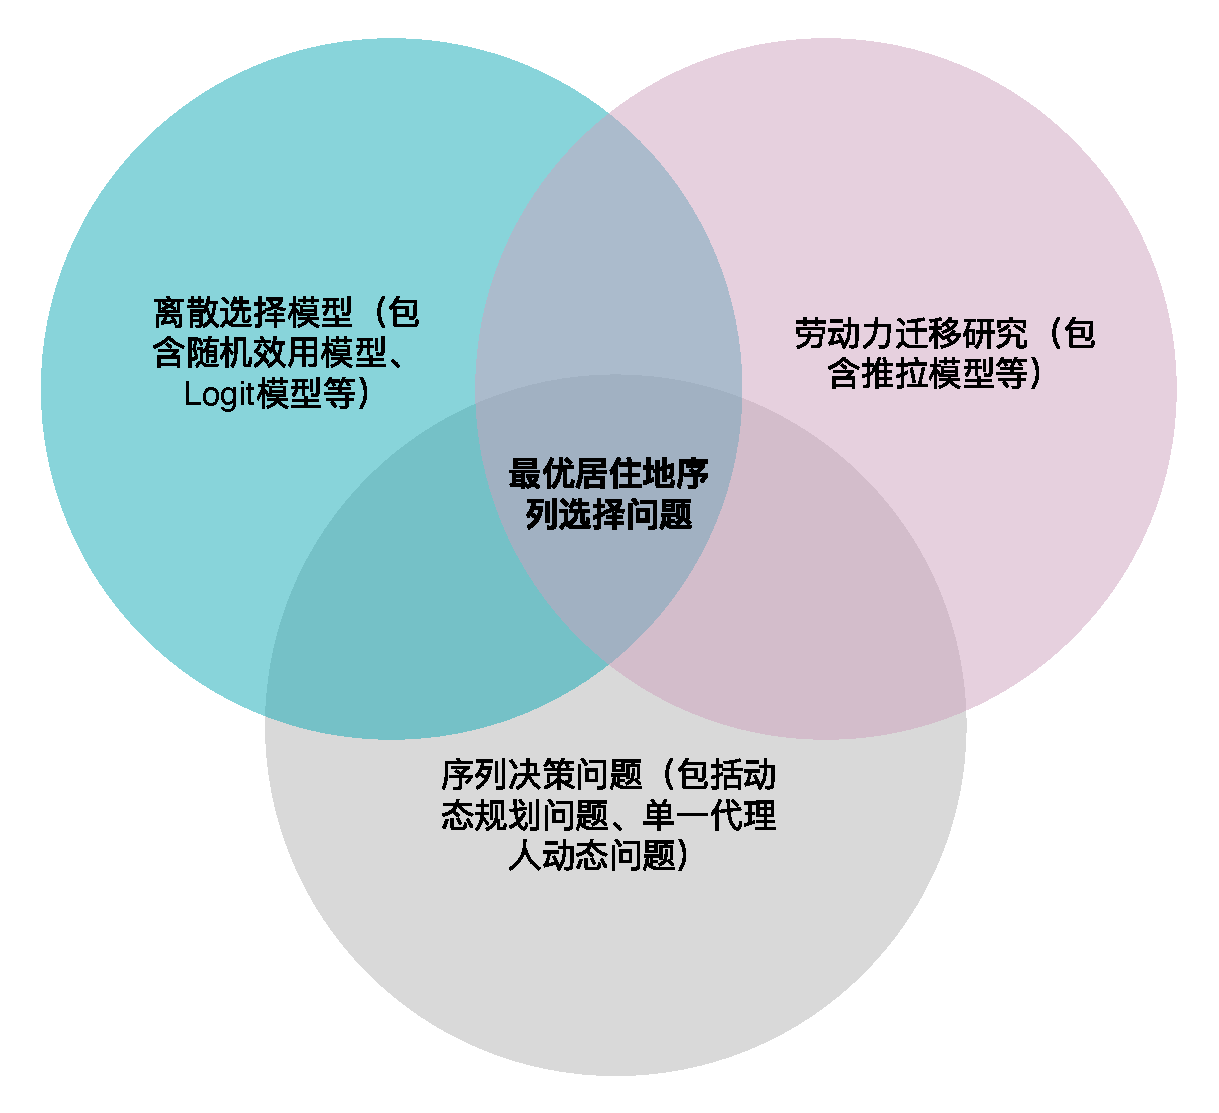
\includegraphics[width=0.65\textwidth]{images/optimal_residential_sequence.drawio.pdf}
\label{fig:最优居住地序列选择问题的理论来源venn diagram}
\end{figure}
























% ---------------------------------------- 理论模型 ----------------------------------------
\chapter{理论模型}

劳动力流动问题本质上极为复杂。经过前述分析,我们认识到,劳动力流动和迁移不应被简单地视为一次性经济活动,而应被理解为贯穿个体整个生命周期的持续决策过程。
假设决策者\footnote{文章中出现的个体指可以独立做出决策的经济单位,其形式可能为个人,也可能为家庭。为了消除歧义,后续将使用“决策者”一词替代。}是理性的,能够在多个地理位置之间进行自主选择。每个地区都对应一个独特的、排他性的效用流 (utility flow)。决策者在进行迁移时,需要承担相应的迁移成本。
当决策者做出迁移决策后将承担相应的迁移成本。
这意味着劳动力流动的本质是一个投资决策。
决策者放弃当前的确定性(如本地工作),投资于一个充满不确定性但可能回报更高的未来(去大城市)。成本不仅是路费和短期收入损失,更是社会网络的断裂、制度性歧视以及巨大的心理压力。收益也不仅是更高的工资,更是子女的未来、更广阔的职业平台和个人价值的实现。
决策者在不同阶段根据自身状况和外部环境变化,不断权衡是否迁移、迁移到何处,以及迁移后如何实现自身利益最大化。

本文通过DDCM框架构建了一个迁移决策模型,来刻画劳动力在不同阶段的定居与迁移选择,其必要性主要体现在以下三点。
首先,静态模型通常假设个体基于当期特征作出一次性选择,忽视了人力资本积累、迁移经验、信息更新等动态因素对后续迁移意愿的影响。然而,在现实中,迁移意愿会随着年龄增长、技能提升、家庭结构变化而不断调整,这种时间路径依赖是静态框架无法捕捉的。  
其次,DDCM可以更有效地处理不可观测的个体异质性。现实中的决策者在风险偏好、流动成本感知等方面存在差异,这些特质既难以直接观测,又会与迁移行为相互作用,形成复杂的内生机制。静态方法往往将这些差异视为随机误差处理,从而掩盖了其结构性影响;而DDCM可以在动态结构中引入状态变量与潜在类型(latent types),从而更系统地识别和解释这类异质性。  
再次,与空间均衡方法相比,DDCM不依赖于市场已经达到长期均衡的假设,而是能够刻画非均衡过渡过程与前瞻性预期。空间均衡模型擅长解释长期劳动力配置与区域间工资、房价的均衡关系,但无法描述短期内政策冲击、经济波动或信息变化对个体迁移决策路径的影响。DDCM则通过显式引入跨期预期效用函数,允许个体在决策中权衡即时收益与未来回报,从而能够在非均衡环境下分析政策效应与行为调整过程。 
为此,本章将以更贴近现实的建模方式分析迁移行为及其背后的逻辑。

\section{模型的基本设定}

本文考虑一个人口总量恒定的封闭经济体,人口流动仅发生在国内各地区之间。
经济体由 $m$ 个离散地区组成,形成迁移网络$\mathcal{C} = \{1,2,\dots,m\}$,这也是个体决策者的行动空间。
各区域拥有固定的地理边界和空间关系,每个地区连通且可达,迁移连通性由$m \times m$列的邻接矩阵$Adj=[j_{xy}\in\{0,1\}]$刻画。 
不同的区域都具有独特的地区特征,这包括经济特征与非经济特征等,每个地区的特征随时间动态变化,会影响个体的迁移决策。
各地区的工资由本地劳动力市场决定。
时间被划分为离散的时期$t=\{0,1,2,\ldots,t,t+1,\ldots\}$。理性决策者$i$获取效用,在每个时期以效用最大化为目标做出迁移决策。地区特征(如工资、就业机会)、经济状况和政策随时间变化,影响个体的预期和决策。

本模型的一个核心特征是引入了中国的户籍制度。我们假设个体$i$的户口所在地$h_i$在其出生时确定且终身不变。当个体选择的居住地$j_t$与其户籍地$h_i$不一致时(即人户分离),其在获取公共服务、社会福利等方面会面临障碍,从而产生负效用。反之,居住在户籍地则无此惩罚。户籍制度对于决策者的影响效果如图\ref{fig:户籍制度造成影响的途径}所示。
\footnote{
一个自然的问题是:在存在诸多摩擦的经济体中,人口流动是否会最终停止?在经典的劳动力自由流动模型中,地区间工资差异会因套利行为而趋于收敛。然而,在本模型中,地区间的非经济舒适度差异、以及个体对不同地区的异质性偏好,是驱动持续流动的根本动力。更重要的是,我们引入的户籍制度、家乡溢价和多维度的迁移成本,恰恰是对劳动力自由流动的制约,这些摩擦的存在解释了为何现实中地区间的巨大差异能够长期持续存在,从而使模型的动态迁移过程更贴近现实。
}

\begin{figure}[!ht]
\centering
\caption{户籍制度造成影响的途径}
\label{fig:户籍制度造成影响的途径}
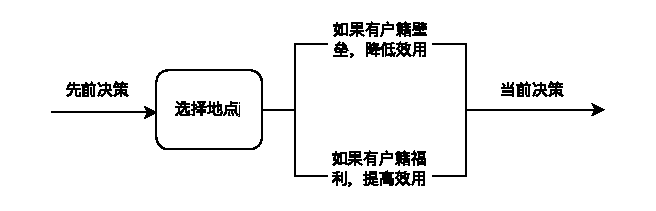
\includegraphics[width=0.8\textwidth]{images/户口影响.drawio.pdf}
\end{figure}

为了处理模型中的跨期决策问题,同时保持计算上的可行性,本文遵循了动态离散选择文献中的一个标准做法,假设存在一个完美的资本市场,个体可以在固定利率下自由借贷。此外,我们假设个体的效用函数对于由收入带来的消费是线性的,即收入的边际效用 $\alpha_w$ 是一个常数。在此假设下,家庭的资产持有对一次性迁移决策的边际影响可被忽略,因此模型中未将资产作为显式状态变量。

一个理性的决策者代理人的决策遵循一个马尔可夫决策过程 (Markov Decision Process, MDP)。决策者在$T$期离散生命周期内选择最优居住地序列。令$j_t \in \mathcal{C}$表示第$t$期的居住地选择,决策者的那么完整的选择序列可表示为$\mathcal{J}=\{j_1, j_2 ,\dots,j_T\}$。典型的居住地选择模式如表格\ref{tab:居住地选择序列可能的形式}所示。

\begin{table}[!ht]
\centering
\begin{tabular}{@{}ll@{}}
\hline
\multicolumn{1}{c}{\textbf{个体流动形式}} & \multicolumn{1}{c}{\textbf{居住地选择序列}}    \\ \midrule
\begin{tabular}[c]{@{}l@{}}\textbf{长期定居}:决策者在特定时间段内总是\\ 停留在同一个地区\end{tabular}                          & $\mathcal{J}=\{\dots, 1,1,1,1,1,\dots\}$ \\
\begin{tabular}[c]{@{}l@{}}\textbf{单向迁移}:如果 $j_p \neq j_q, \forall p\neq q$,那么\\ 个体就进行了迁移\end{tabular} & $\mathcal{J}=\{\dots, 1,2,3,4,5,\dots\}$ \\ 
\textbf{回流迁移}:返回到先前居住过的地区                      & $\mathcal{J}=\{\dots, 1,2,2,1,1,\dots\}$ \\ \bottomrule
\end{tabular}
\caption{居住地选择序列可能的形式}
\label{tab:居住地选择序列可能的形式}
\end{table}


在每一时期 $t$ 的决策时刻,一个理性代理人$i$ 已知其上一期所在地点 $l_{i,t-1}$、户籍 $h_i$ 等信息,并据此选择本期的居住地 $j_t\in\mathcal C$。我们将个体在时期 $t$ 决策前的全部相关信息定义为状态向量 $x_{it}$:
\begin{equation}
x_{it} = \bigl(a_{it},\; l_{i,t-1},\; h_i,\; H_{it},\; \{\nu_{ik}\}_{k\in H_{it}},\; \eta_i,\; K_t\bigr),
\end{equation}
其中$a_{it}\in \{A_{min},\dots,A_{max}\}$为代理人的年龄;$H_{it}=\{l_{i0},\dots,l_{i,t-1}\}$ 为个体已到访的地点集合(历史记录),$\{\nu_{ik}\}_{k\in H_{it}}$ 为个体已知的个体–地点匹配值,$\eta_i$ 为个体固定效应,$K_t$ 为宏观状态。
在时期 $t$,个体在观测到自身状态 $x_{it}$ 以及当期的随机效用冲击 $\{\zeta_{itj}\}_{j\in\mathcal{C}}$ 后,做出居住地选择 $j_t$。

在时期$t$,个体$i$若选择居住在潜在的地点$j$处,
\footnote{
  $j$是一个泛指的、潜在的选项,是一个哑变量或者索引。而$j_t$一个已实现的、实际的选择,是一个随机变量,其值是在时期 t 做出的具体决策结果。此处切换为$j$是为了泛化模型。
}
其获得的总效用以McFadden效用函数形式给出:
\begin{equation}
  \tilde{u}_{it}(j, x_{it}, \theta) = u_{it}(j, x_{it}, \theta) + \zeta_{itj}
  \label{eq:地区效用函数}
\end{equation}
其中$u_{it}(j, x_{it}, \theta)$为可观测的效用流,$\theta$是需要估计的结构性参数;
$\zeta_{itj}$为不可观测的效用冲击,是在任意时期和地点都独立同分布的随机扰动项,服从Type I极值分布(Gumbel分布),且与状态变量$x_t$无关。

居民的基础效用由货币性收入、城市宜居度、家乡溢价减去迁移成本组成。
为了捕捉驱动迁移决策的关键因素,可观测效用流$u_t$函数的具体形式设定如下:
\begin{equation}
\begin{split}
     u_{it}(j, x_{it}; \theta) = & \underbrace{ U^{\text{income}}(w_{itj} | w_{it}^{ref}) }_{\text{对经济收入的预期管理}} + \underbrace{\sum_s \alpha_s \cdot y_{sj}(K_t)}_{\text{地区舒适度}} + \underbrace{\alpha_{home} \cdot I(j=h_i)}_{\text{家乡溢价}} \\
    & - \underbrace{\text{HukouPenalty}(j, h_i, K_t)}_{\text{户籍制度惩罚}} - \underbrace{\kappa_{it}(j, x_{it})}_{\text{迁移成本}} + \underbrace{\xi_{ij}}_{\text{偏好匹配}}
\end{split}
\label{eq:确定性效用函数}
\end{equation}


该函数由六个部分构成:
\begin{enumerate}
  \item 对于经济收入的期望管理:$U^{\text{income}}(w_{itj} | w_{it}^{ref})$,当个体在地区 $j$ 获得的工资 $w_{itj}$ 与预期收入锚点进行比较,得到的一种满足感或者落差感。
  \item 地区舒适度 (Amenities):由气候、公共服务等一系列非经济因素 $y_{sj}$ 决定的地区吸引力,$\alpha_s$ 是其边际效用。
  \item 家乡溢价 (Home Premium):当个体居住在户籍地 $h_i$ 时,获得的额外心理效用 $\alpha_{home}$。这是一个只在家乡生效的拉力。
  \item 户籍制度惩罚 (Hukou Penalty):当个体居住在非户籍地时,由于制度壁垒产生的负效用。这是一个在所有非家乡地区生效的“推力”。
  \item 迁移成本 (Migration Cost):如果个体发生迁移(即 $j \neq l_{i,t-1}$),需要支付的一次性成本 $\kappa_{it}$。
  \item 非经济偏好匹配: 个体 $i$ 对地区 $j$ 的一种持久的、非货币化的情感或文化契合度 $\xi_{ij}$。与收入匹配项 $\nu_{ij}$ 类似,其真实值只有在个体访问过地区 $j$ 后才能知晓。它捕捉了除收入外,个体与地区之间的特殊化学反应。
\end{enumerate}

下文将对效用中货币收益项 $w_{itj}$ 进行结构化建模,以便将个体工资形成机制与迁移选择共同识别。

\section{收入效用函数}

本模型引入了基于前景理论的损失厌恶机制,以提供了一个全新的、有别于传统迁移成本的机制来解释人们的迁移预期。假设个体的效用并非直接来源于其收入的绝对水平,而是来源于其实际收入与其参照点之间的比较。因此,我们将效用函数中的收入项从线性的 $α_w * w_{itj}$ 修正为 $U^{\text{income}}(w_{itj} | w_{it}^{ref})$。

\begin{equation}
U^{\text{income}}(w_{itj}, w_{it}^{ref}) =
\begin{cases}
\alpha_w (w_{itj} - w_{it}^{ref}) & \text{if } w_{itj} \ge w_{it}^{ref} \quad \text{(收益域)} \\
\alpha_w \cdot \lambda \cdot (w_{itj} - w_{it}^{ref}) & \text{if } w_{itj} < w_{it}^{ref} \quad \text{(损失域)}
\end{cases}
\label{eq:收入效用函数}
\end{equation}

这一设定意味着效用来自于实现的增益和损失。正的收入差距 $(w_itj - w_it^ref)$ 代表了超出预期的成就感,而负的差距则代表了未达预期的失落感。损失厌恶系数$\lambda$则量化了人们"宁可不赚,不可赔“的心理,即损失带来的负效用要大于等量收益带来的正效用。$\alpha_w$ 依然是收入的(收益域)边际效用,预期为正。

决策者的收入函数由多种因素组成。个体决策者$i \in \mathcal{N}$在时期$t$、地点$j$的收入设定为以下函数形式:
\begin{equation}
    w_{itj}=\mu_j(K_t)+G(X_i, a_{it}, t)+\eta_i+\nu_{ij}+\varepsilon_{itj}
  \label{eq:收入函数}
\end{equation}


\begin{enumerate}
  \item $\mu_j(K_t)$ 为地点 $j$ 的基准薪资水平,代表地区的经济基本面,如生活成本、区域产业聚集效应(如北京的传媒业、山西的采矿业)、政策红利(税收减免、人才补贴)等结构性特征,是所有在该地点个体的工资基准,其与个体无关,仅随宏观状态 $K_t$ 变化。
  \item 生命周期收入 $G(X_i, a_{it}, t)$捕捉由个体年龄(人力资本积累)决定的收入部分,是人力资本积累的代表。在传统的设定中,$G(\cdot)$ 通常被假设为一个关于年龄的二次多项式和线性控制变量的组合。然而,为了避免因函数形式误设而导致的偏误,我们在实证估计中将采用更灵活的方法。具体而言,我们将使用机器学习模型来非参数地估计 $G(\cdot)$ (详见 \ref{sec:ml_plugins} 节
  \item 个体固定效应 $\eta_i$代表个体不随地点改变的固有能力或特质,如先天能力、家庭背景等。
  \item 个体-地区匹配效应$\nu_{ij}$捕捉了特定个体 $i$ 在特定地区 $j$ 的生产力特殊加成(如技能需求匹配、文化契合度),代表相同技能劳动者在不同地区的收入差异。该值在个体首次进入地区 $j$ 时实现(从一个分布 $F_\nu(0, \sigma_{\nu,jt}^2)$ 中抽取),此后在该地区停留期间保持不变,但迁移到新地区$k$ 时会生成新的 $\nu_{ik}$。
  \item 暂时性随机效应$\varepsilon_{itj}$代表短期波动或随机扰动项,服从零均值正态分布的当期随机工资冲击,代表了不可预测的短期波动(如临时绩效波动、经济冲击)。
\end{enumerate}

假设个体-地区匹配效应分布$F_\nu(0, \sigma_{\nu,jt}^2)$的方差(或离散支撑点的范围)是随信息渠道变化的:
$$\nu_{ij} \sim F_\nu(0, \sigma_{\nu,jt}^2)$$

其中,方差 $\sigma_{\nu,jt}^2$ 的函数形式为:
$$\sigma_{\nu,jt}^2 = \exp(\delta_0 - \delta_1 \cdot \text{Internet}_{j,t})$$
其中$\delta_0$ 和 $\delta_1$ 是待估参数。$\delta_1$ 是核心参数,我们预期 $\delta_1 > 0$。这意味着,当一个地区的互联网普及率 $Internet_{j,t}$ 越高时,你去那里之前面临的收入不确定性 $\sigma_{\nu,jt}^2$ 就越低。

这对模型意味着当个体考虑迁移到一个新的、互联网不发达的地区 $j$ 时,他面临的 $\nu_{ij}$方差很大。这意味着工资可能是惊喜(抽到很高的 $\nu$),也可能是惊吓(抽到很低的 $\nu$)。风险厌恶的个体会因此不愿意去。
当考虑迁移到一个新的、互联网发达的地区 $k$ 时,$\nu_{ik}$的方差较小。个体对去那里能拿到的工资更有把握,决策的不确定性降低,从而更愿意迁移。


同时,正因为假设$\varepsilon$服从期望为0的正态分布,若在数据中观测到个体$i$在时期$t$的写为$j_t$,其实际工资为 $w_{itj}^{\mathrm{obs}}$,可知其条件密度为
\begin{equation}
\mathcal{L}{i,t}^{\text{wage}} = \frac{1}{\sigma\varepsilon}\phi\left(\frac{w_{it,j_t}^{\mathrm{obs}}-\mu_{j_t}(K_t)-G(X_i,a_{it})-\eta_i-\nu_{ij_t}}{\sigma_\varepsilon}\right)
\label{eq:工资自然贡献}
\end{equation}
其中 $\phi(\cdot)$ 为标准正态密度,该方程为处于地点$j$的个体$i$在时期$t$的收入函数的密度函数$\Psi_{itj}$。这是个体 $i$ 在时期 $t$ 于地区 $j$ 的工资观测值对总似然函数的贡献。

\section{户籍惩罚、家乡溢价与地区舒适度}

真实世界中户籍制度带来的效应是多维度的、有异质性的,为了细致刻画这种复杂影响,本文因此假设了一个分层的、与地区特征互动的户籍效应模型:
\begin{equation}
    \begin{split}
        \text{HukouPenalty}(j, h_i, K_t) ={}& I(j \neq h_i) \cdot \bigl[ \theta_{\text{base}}(P_j) + \theta_{\text{edu}} \cdot \text{Edu}(j) \\
        & + \theta_{\text{health}} \cdot \text{Health}(j) + \theta_{\text{house}} \cdot \text{HousingPrice}(j) \bigr]
    \end{split}
\label{户籍惩罚函数}
\end{equation}
其中:
\begin{enumerate}
  \item 指示函数 $I(j \neq h_i)$:表示只有在人户分离时,惩罚才生效。
  基础惩罚 $\theta_{base}(P_j)$:这不是一个单一参数,而是一个依赖于目标省份 $P_j$ 的参数。例如,可以设定 $\theta_{base}(\text{北京}) > \theta_{base}(\text{安徽})$。这捕捉了不同地区户籍政策的宽松程度。在估计时,你可以为每个省份(或几类省份,如一线城市、二线城市、其他)估计一个不同的基础惩罚。
  \item 与公共服务互动的惩罚:$\theta_{edu} \cdot \text{Edu}(j)$: 户籍惩罚的大小与该地区的教育质量(如重点高中比例)成正比。教育资源越好的城市,没有本地户口的孩子上学越困难,因此惩罚越大。预期 $\theta_{edu} > 0$。
  \item $\theta_{health} \cdot \text{Health}(j)$:与该地区医疗水平(如三甲医院数量)成正比。医疗越好的地方,医保报销的地区差异带来的损失越大。预期 $\theta_{health} > 0$。
  \item 与生活成本互动的惩罚:$\theta_{house} \cdot \text{HousingPrice}(j)$: 与该地区的房价等生活成本指标互动。很多城市的购房资格与户口或社保年限挂钩,房价越高,这种限制带来的机会成本就越大。预期 $\theta_{house} > 0$。
\end{enumerate}


户籍效应的机制扎根于制度性、政策性的进入壁垒。它源于公共服务(教育、医疗)的排他性、购房购车资格的限制等。
这是一个推离异乡(Push Factor)的力。
它是一种负向效用(成本或惩罚),在个体身处任何非户口所在地时都会承受。该变量对所有 $m-1$ 个非户口所在地都生效,且惩罚大小因地而异。户籍效应可以通过观察个体在不同城市间的选择来识别。例如,如果两个城市A和B工资和舒适度相似,但城市A的户籍管制更严(公共服务更好),那么需要一个更高的工资差异才能吸引无户口者去A城。这个补偿性工资差异就反映了户籍惩罚的大小。

本文同时还在模型中假设了家乡溢价效应 ($\alpha_{home} \cdot I(j=h_i)$),这个变量不同于户籍效应,是一个拉回家乡(Pull Factor)的力,是一种正向效用,只在个体身处家乡时才会获得。该变量刻画的是心理、社会、文化层面的情感依恋,是对家乡非理性偏好的量化。它源于家庭纽带、朋友圈、熟悉的文化环境等。只对一个特定地点(家乡 $h_i$)生效。家乡溢价效应变量通过观察个体即使在面临更好的外地经济机会时,依然选择留在或返回家乡的行为来识别。

模型中的地区舒适度和户籍惩罚可能包含相同的地区特征变量,如教育和医疗资源。这并非重复计算,而是为了识别这些资源在效用层面上的两种不同渠道。

以教育变量为例,在地区舒适度中舒适度项 $\alpha_s^{Edu} \cdot \text{Edu}(j)$ 代表教育资源作为一种公共品带来的普遍效用。一个地区教育好,所有人(无论有无户口)都会觉得这个地方有文化氛围、重视下一代,从而增加其作为居住地的吸引力。这是一种对所有决策者生效的环境效应。而在户籍惩罚中,$\theta_{\text{Edu}} \cdot \text{Edu}(j)$代表教育资源作为一种排他性服务带来的效用损失。一个地区教育越好,没有户口的人在享受这种服务时面临的壁垒就越高(比如子女不能参加本地高考),因此他们感受到的惩罚就越大。这是一种只针对人户分离决策者的准入成本。

模型正是通过比较户籍人口与非户籍人口对这些资源的不同反应,来分别识别参数 $\alpha_s^{Edu}$ 和 $\theta_{\text{Edu}} $的。


以上效应结合在同一个模型中,是解释中国劳动力流动谜题(如大量回流、城乡差距长期存在)的关键且独立的机制。


\section{迁移成本}

决策者$i$的迁移成本$\kappa$设定为以下函数形式:
\begin{equation}
\begin{split}
\kappa_{it}(j, x_{it}) = & I(j \neq l_{i,t-1}) \cdot \biggl[ \gamma_{0\tau} + \gamma_1 D(l_{i,t-1}, j) - \gamma_2 I(j \in \text{Adj}(l_{i,t-1})) \\
    & - \gamma_3 I(j \in H_{it}) + \gamma_4 a_{it} - \gamma_5 n_j(K_t) \biggr]
\end{split}
\label{eq:迁移成本函数}
\end{equation}

其中,指示函数 $I(j \neq l_{i,t-1})$ 确保了原地停留者成本为零。成本构成包括:
\begin{enumerate}
  \item $\gamma_{0\tau}$: 与个体类型 $\tau$ 相关的固定成本,随个体类型哑变量 $\tau$ 变化,用以捕捉“恋家型”与“闯荡型”等未观测到的异质性。例如定居型个体的 $\gamma_{0\tau}$ 极高,几乎禁止迁移;流动型个体的 $\gamma_{0\tau}$ 较低,更易迁移。不同类型的群体分布由对应的概率$\pi_\tau$给出,并且满足$\sum\limits_{\tau}^{} \pi_\tau=1$。

  \item $\gamma_1 D(l_{i,t-1}, j)$: 与物理距离相关的线性成本(以大圆距离衡量)。

  \item $-\gamma_2 I(j \in \text{Adj}(l_{i,t-1}))$: 迁移到相邻地区的成本折扣,相邻地区迁移可能因文化相似、信息透明或交通便利而成本更低。

  \item $-\gamma_3 I(j \in H_{it})$: 回流迁移的成本折扣,因为返回曾居住过的地区,社会网络和适应性成本较低。

  \item $\gamma_4 a_{it}$: 年龄越大,迁移的心理或生理成本越高,这是随年龄增长而增加的迁移阻力。

  \item $-\gamma_5 n_j(K_t)$: 迁入地人口规模带来的成本减免效应,反映了更大城市网络带来的便利。目标地区人口规模 $n_j$ 越大,迁移成本减少 $\gamma_5 n_j$。这是因为大规模地区可能有更多潜在支持(如亲友网络、服务机构),减少安家难度,从而降低迁移成本($\gamma_5 > 0$),符合引力模型中人口规模吸引迁移的经典结论。  
\end{enumerate}




迁移成本中参数的经济含义如表格\ref{tab:迁移成本参数释义}所展示。
\begin{table}[!ht]
  \centering
  \caption{迁移成本参数释义}
  \label{tab:迁移成本参数释义}
  \begin{tabularx}{\textwidth}{@{}llX@{}}
    \toprule
    \multicolumn{1}{c}{\textbf{参数符号}} & \multicolumn{1}{c}{\textbf{参数含义}} & \multicolumn{1}{c}{\textbf{参数意义}} \\ \midrule
    \multicolumn{1}{c}{$\gamma_{0\tau}$} & 类型异质效应 & 捕捉不同类型的异质性,可以解释为何有些人从不迁移,识别“定居型”人群可针对性地设计激励措施(如搬迁补贴)。\\ 
    \multicolumn{1}{c}{$\gamma_1$} & 物理迁移成本 & 个体与其携带物必然因为物理法则而产生运输成本。 \\ 
    \multicolumn{1}{c}{$\gamma_2$} & 相邻地区效应 & 反映地理邻近性的普遍优势。 \\ 
    \multicolumn{1}{c}{$\gamma_3$} & 历史地区效应 & 返回历史地区因熟悉度获得折扣,体现路径依赖。 \\ 
    \multicolumn{1}{c}{$\gamma_4$} & 年龄障碍效应 & 针对不同年龄群体制定差异化迁移政策(如青年人才引进计划)。\\ 
    \multicolumn{1}{c}{$\gamma_5$} & 规模成本效应 & 大地区吸引力不仅体现在经济机会(如工资 $\mu_j$),也直接降低迁移成本。\\ \bottomrule
  \end{tabularx}
\end{table}

迁移成本不仅影响当前选择,也会改变 $H_{it}$ 与未来可获得的匹配信息,从而通过状态转移影响未来效用。

\section{状态转移概率}



状态转移概率 $p(x_{i,t+1}|x_{it}, j_t)$ 描述了系统如何从当前状态演化至下一期状态。值得强调的是,本模型通过将历史居住地集合 $H_{it}$ 和已知的匹配值 $\{\nu_{ik}\}_{k\in H_{it}}$ 纳入状态向量 $x_{it}$,从而内生化了路径依赖。这意味着,尽管状态转移本身遵循马尔可夫属性(即 $p(x_{t+1}|x_t, j_t, x_{t-1}, \dots)$ 简化为 $p(x_{t+1}|x_t, j_t)$),但由于过去已经被编码在现在$x_{it}$之中,个体的决策实质上是历史依赖的。这种设定既保持了马尔可夫决策过程的分析便利性,又能够捕捉学习效应和回流迁移等复杂的动态行为,是本模型的一个关键特征。


具体而言,由于状态变量是多维的,本文将其设置为:

\begin{itemize}
    \item 年龄: $a_{i,t+1} = a_{it} + 1$ (确定性转移)
    \item 上一期位置: $l_{i,t} = j_t$ (确定性转移)
    \item 户口所在地: $h_i$ (不变)
    \item 个体固定效应: $\eta_i$ (不变)
    \item 历史居住地集合: $H_{i,t+1} = H_{it} \cup \{j_t\}$ (确定性转移)
    \item 宏观状态: $K_{t+1} \sim p(K_{t+1}|K_t)$ (随机转移,通常假设为一阶马尔可夫过程)
    \item 已知的匹配值: 
\end{itemize}  

$$ p(\{\nu_{ik}\}_{k \in H_{i,t+1}} | \{\nu_{ik}\}_{k \in H_{it}}, j_t) = \begin{cases} \delta(\{\nu_{ik}\}_{k \in H_{i,t+1}} - \{\nu_{ik}\}_{k \in H_{it}}) & \text{if } j_t \in H_{it} \\ f_\nu(\nu_{ij_t}) & \text{if } j_t \notin H_{it} \end{cases} $$
这样的设定意味着,如果 $j_t$ 是一个已经去过的地方 ($j_t \in H_{it}$),那么个体不会学到新的信息,已知的匹配值集合不变。这里的 $\delta(\cdot)$ 是狄拉克函数,表示这是一个确定性的转移。
如果 $j_t$ 是一个新的地方 ($j_t \notin H_{it}$),个体在选择 $j_t$ 后,便会获知新的匹配值 $\nu_{ij_t}$。这个新值是从分布 $F_\nu$ 中抽取的,其概率密度为 $f_\nu(\cdot)$。而已知的其他匹配值保持不变。这个新信息将被纳入下一期的状态向量 $x_{i,t+1}$ 中,从而影响其未来的决策。


\section{条件选择概率函数}

个体的目标是选择一个居住地序列 $\mathcal{J}^* = \{j_1^*, \dots, j_T^*\}$ 以最大化其终身期望折现效用,即:
\begin{equation}
  \max_{\mathcal{J}=\{j_1,j_2,\ldots,j_T\}} \mathbb{E} \left[ \sum_{t=1}^{T} \beta^{t-1} \tilde{u}_{it}(j_t,x_{it}) \right]
\end{equation}

该问题可通过贝尔曼方程描述。令 $\beta \in (0,1)$ 为折现因子。在第 $t$ 期、状态为 $x_t$ 时,选择潜在地区 $j$ 的期望折现总效用(不含当期的随机冲击)可以用选择特定价值函数(Choice-Specific Value Function)表示:
\begin{equation}
v_{it}(x_{it}, j) = u_{it}(j, x_{it}; \theta) + \beta \cdot \mathbb{E} \left[\bar{V}_{i,t+1}(x_{i,t+1}) \mid x_{it}, j \right]
\end{equation}
其中
\begin{equation}
\bar{V}_{it}(x_{it}) = \mathbb{E}_{\zeta} \left[ \max_{k \in \mathcal{C}} \{ v_{it}(x_{it}, k) + \zeta_{ik,t} \} \right]
\end{equation}
为期望价值函数 (Expected Value Function),即在状态 $x_{t+1}$下,对所有可能随机扰动 $\zeta$ 取期望后的长期效用,是代理人知道$x_t$但在抽取当期随机冲击$\zeta_t$之前的期望效用。

在每一期,当随机冲击向量 $\{\zeta_{ij,t}\}_{j \in \mathcal{C}}$实现后,理性代理人会选择使其总效用最大化的地区 $j_t^*$:
\begin{equation}
j_{it}^* = \arg\max_{j \in \mathcal{C}} { v_{it}(x_{it}, j) + \zeta_{ij,t} }
\end{equation}

代理人在选择集$\mathcal{C}$中选择行动$j$的概率为条件选择概率(Conditional Choice Probability, CCP)函数,可以表示为:
\begin{equation}
\begin{split}
    P(j_t|x_t,\theta)&=Prob(\tilde u_j > \tilde u_k, \forall k \neq j)
    \\&=Pr(u_j+\zeta_j>u_k+\zeta_k, \forall k \neq j)
    \\&=Pr(\zeta_k-\zeta_j<u_j-u_k, \forall k \neq j)
\end{split}  
\label{eq:C中地点选择j的概率}
\end{equation}


根据\textcite{rustOptimalReplacementGMC1987} 以及\textcite{hotzConditionalChoiceProbabilities1993} 的开创性工作,由于 $\zeta_j$ 独立同分布且服从 I 型极值分布(尺度为1),CCP可以写为softmax函数形式:
\begin{equation}
P(j_t = j \mid x_{it}; \theta) = \frac{\exp(v_{it}(x_{it}, j))}{\sum_{k \in \mathcal{C}} \exp(v_{it}(x_{it}, k))}
\label{eq:地点选择概率}
\end{equation}
这极大地优化了动态规划问题中期望值的计算。
并且由于sotfmax函数输出的概率分布是平滑的,有利于策略迭代的稳定性。

图\ref{fig:migration_flow_resized2} 展示了一个动态规划决策过程。在离散周期$t$结束时或者下个周期$t+1$即将开始时,决策者根据在抽取到的随机收益冲击$\zeta$和状态转移概率$p(x_{t+1}|x_t,j_t)$双重不确定性的影响下通过Bellman方程做出决策,进入下一个周期$t+1$后获得该期的效用$\tilde u_{t+1}$。

\begin{figure}[!ht]
\centering
\caption{动态离散选择模型下的劳动力迁移决策流程图}
\label{fig:migration_flow_resized2}
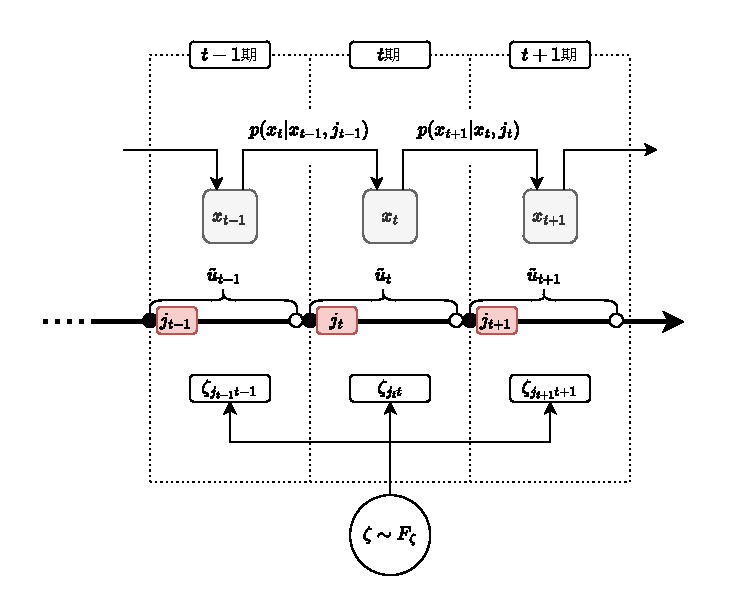
\includegraphics[width=0.9\textwidth]{images/dynamicsequence2.drawio.pdf}
\end{figure}


为保持可读性,文中所有符号均按表 \ref{tab:notation} 给出含义。
\begin{table}[ht]
\centering
\caption{符号说明}\label{tab:notation}
\begin{tabularx}{\textwidth}{lX}
\toprule
符号 & 含义 \\
\midrule
$i,t,j$ & 个体、时间、地点索引 \\
$a_{it}$ & 年龄 \\
$l_{i,t-1}$ & 时期 $t$ 决策前的上一期地点 \\
$h_i$ & 户籍地 \\
$H_{it}$ & 已到访地点集合(历史) \\
$w_{itj}$ & 工资(货币性收入) \\
$\mu_j(K_t)$ & 地点基准工资(随宏观态 $K_t$ 变化)\\
$\nu_{ij}$ & 个体—地点匹配效应\\
$\varepsilon$ & 工资的暂态效应\\
    $\eta_i$ & 个体固定效应 \\
    $\kappa_{it}(j,\cdot)$ & 迁移成本 \\
    $\mathrm{HukouPenalty}(\cdot)$ & 户籍惩罚 \\
    $\zeta_{ij,t}$ & 个体-地点-时间特定的随机效用冲击(Type I EV) \\
    $\theta=(\gamma,\alpha \dots)$ & 待估结构参数向量\\
    $\beta$ & 外生给定的折现因子 \\
\bottomrule
\end{tabularx}
\end{table}



\section{劳动力迁移决策}

综合以上设定,个体是否从地区 $j$ 迁移到地区 $k$ 的决策,本质上是一个对各项利弊的权衡。个体选择迁移到 $k$ 的条件是 $v_{it}(x_{it}, k) + \zeta_{k,t} > v_{it}(x_{it}, j) + \zeta_{j,t}$。忽略未来期望价值的差异,仅看当期效用,这一决策可以直观地理解为:
\begin{equation}
\begin{split}
  & \underbrace{ \left( \alpha_w (w_k - w_j) + (\text{Amenity}_k - \text{Amenity}_j) + \dots \right) }_{\text{地区 k 相对于 j 的吸引力增益}} \\
  & > \underbrace{\kappa_{j \to k}}_{\text{迁移成本}} + \underbrace{ (\text{HukouPenalty}_k - \text{HukouPenalty}_j) }_{\text{户籍惩罚变化}} + \underbrace{ (\text{HomePremium}_k - \text{HomePremium}_j) }_{\text{家乡溢价变化}} \\
  & + \underbrace{ (\zeta_{j,t} - \zeta_{k,t}) }_{\text{随机偏好冲击}}
\end{split}
\label{eq:迁移motivation_revised}
\end{equation}
目标地区带来的经济与非经济收益的提升,必须足以克服迁移的直接成本、可能的制度性惩罚增加、以及放弃家乡溢价的损失。

至此,模型完整地刻画了一个理性个体,在有限生命周期和多重约束下,如何动态地在迁移网络$\mathcal{C}$中选择其最优居住地序列 $\mathcal{J}^*$。该框架允许个体进行多次、可逆的迁移,从而能够灵活地解释现实世界中复杂的劳动力流动模式。这种对劳动力迁移的自由性的刻画,与现实世界中的行为是融洽的。




% ---------------------------------------- 实证部分 ----------------------------------------
\chapter{实证处理}

将前述构建的动态迁移决策模型付诸实证检验,面临着重大的计算挑战。
动态规划本身就面临着维度诅咒带来的计算资源稀缺问题,传统方法使用两步法来解决。但当模型中个体决策依赖于多维度的、持久性的未观测异质性(如个人能力$\eta_i$或潜在类别$\tau$),在两步估计法中第一步估计的 CCPs 容易产生偏误,并且误差无法在第二步中完全纠正。这是因为从数据中估计的CCP是所有异质类型个体行为的加权平均,无法直接用于识别特定类型的结构参数。

为此本文将 CCPs 的计算内嵌在固定嵌套点(Nested Fixed Points, NFXP)的内循环中,并通过期望最大化(Expection-Maximization, EM)算法机制动态更新未观测类型的后验概率,从而实现联合估计。这种方法能够避免由分步估计带来的信息丢失,并在有限样本下表现出更好的稳健性。

同时为了减轻这种全解法带来的计算资源压力,我们还设计了专门的多线程并行计算方法。



\section{处理未观测到的异质性}

在结构模型中,合理地刻画个体间无法被直接观测到的异质性,是模型识别和解释力的关键。如果不对此加以识别,模型可能会将个体持久性的偏好或能力差异错误地归因于状态依赖。为此,本研究采用了两种互补的策略来捕捉多维度的未观测异质性:离散因子近似 (Discrete Factor Approximation) 和 有限混合模型 (Finite Mixture Model)。

\subsection{离散化近似}

传统做法通常会对关键随机变量或潜在变量作出明确的分布假设,例如,这类方法虽然具有一定的便利性,但也带来潜在的问题,若真实数据与假设分布存在系统性偏差,模型估计将产生偏误,且这种偏误可能无法通过增加样本量消除。同时,固定的分布假设限制了变量形态,在数据中存在厚尾、偏态、多峰等复杂特征时,传统方法难以捕捉其异质性。

本文不施加正态分布等强参数假设,而是采用灵活的非参数离散化方法进行近似未知分布的变量。我们将这些连续的未知分布用一组有限的支撑点(support points)及其对应的概率(mass points)来表示。
对于任何不知道其分布的 $F$,我们可以找到最佳近似分布 $\hat F$ 来近似。对于连续分布的变量$F$,离散的 $\hat F$ 是一组有限的支撑点组成,每个支撑点都有对应的概率值,即$\{(x_i, p_i)\}, 1 \leqslant i \leqslant N$ 的组合,其中 $x_i$ 是离散点,$p_i$ 是其概率,$N$ 为给定的支持点数。对于每个$q_r, (1\leqslant r \leqslant n )$,计算对应的效用值,用这些有限的效用值来代替连续效用的积分。
通过该处理后,模型变为有限状态的动态规划问题,可以直接构建似然函数并进行最大似然估计。
支撑点位置和权重可以灵活调整,以捕捉厚尾、多峰或非对称等特征。
相比完全非参数估计,离散化将连续分布压缩为有限维参数,既降低计算负担、避免随机噪声,又可通过支撑点直观解释经济含义。

在估计中,我们假设每个支撑点的概率是均等的,需要估计的是支撑点的位置(即值的大小),从而刻画分布的形状和范围。
具体设定如表 \ref{tab:unobserved_heterogeneity_setting} 所示。

\begin{table}[!ht]
  \centering
  \caption{未观测异质性属性的离散化设定}
  \label{tab:unobserved_heterogeneity_setting}
  \begin{tabularx}{\textwidth}{@{}lllX@{}}
    \toprule
    \textbf{异质性来源} & \textbf{符号} & \textbf{设定} & \textbf{经济学含义与识别} \\ 
    \midrule
    \textbf{个体能力} & $\eta_i$ & $N_\eta$个支撑点 & 捕捉不随时间地点改变的个体固有生产力(如天赋、家庭背景)。通过个体在不同地点间持续的平均工资差异来识别。 \\
    \textbf{收入匹配} & $\nu_{ij}$ & $N_\nu$个支撑点 & 捕捉特定个体$i$与特定地区$j$之间的特殊生产力协同效应。通过个体在某地异常高或低的工资,以及试错式的迁移行为来识别。 \\
    \textbf{偏好匹配} & $\xi_{ij}$ & $N_\xi$个支撑点 & 捕捉非经济的、持久的个体-地区情感契合度。识别于那些无法用经济回报解释的、持续的留存或回流选择。 \\
    \textbf{工资波动性} & $\sigma_{\varepsilon,i}$ & $N_\sigma$个支撑点 & 允许不同个体的暂时性工资冲击具有不同的方差,捕捉个体面临的收入不确定性差异(如行业风险)。通过个体工资的时间序列波动幅度来识别。 \\
    \bottomrule
  \end{tabularx}
\vspace{0.5em}
\footnotesize
\end{table}

我们将所有通过离散化近似的未观测属性集合记为:
$$\omega_i = \{\eta_i, \{\nu_{ij}\}_{j \in \mathcal{C}}, \{\xi_{ij}\}_{j \in \mathcal{C}}, \sigma_{\varepsilon,i}\}$$



\subsection{有限混合}

除了上述个体属性的连续性异质性外,本文还假设劳动力群体中存在 $K$ 个离散的、具有异质行为模式的潜在类别,避免了硬性分组(如通过地区、行业、性别等显式变量进行分组)的局限。

这种类别异质性正是由迁移成本函数中的固定成本项 $\gamma_{0\tau}$所引入的。
具体而言,个体 $i$ 属于类别 $\tau \in \{1, 2, \dots, K\}$ 的概率为 $\pi_\tau$,且 $\sum\limits_{\tau=1}^K \pi_\tau = 1$。
属于不同类别 $\tau$ 的个体拥有不同的基础迁移成本 $\gamma_{0\tau}$ 。例如,我们可以预期“恋家型”的 $\gamma_0$ 显著为正且数值较大,而“闯荡型”的 $\gamma_0$ 可能接近于零甚至为负,即使两者面临完全相同的状态变量。

通过这种有限混合设定,模型可以内生地将样本人群划分为几种不同的决策类型,并估计出每种类型的规模$\pi_\tau$及其独特的行为参数$\gamma_{0\tau}$。这不仅极大地增强了模型的拟合优度,也为理解人口流动的复杂模式提供了更丰富的解释维度。在整个估计过程中,个体的类别归属是未知的,我们通过构建混合似然函数对其进行概率加权处理。

上述的两种方法在模型中的作用是互补的。非参数离散化侧重于对迁移决策中的随机冲击分布进行灵活刻画,增强模型在面对未知或复杂分布时的稳健性;有限混合方法则侧重于对劳动力个体层面的结构性异质性进行识别与建模,避免遗漏不可观测分组信息所带来的偏误。通过结合使用这两类方法,模型能够在不牺牲可计算性的前提下,更全面地反映劳动力迁移行为背后的复杂机制。


\section{引入机器学习方法处理滋扰函数} % (fold)
\label{sec:ml_plugins}


本模型的似然函数依赖于对工资条件期望 $\mathbb{E}[w_{itj} | x_{it}]$ 和状态转移概率 $p(x_{i,t+1} | x_{it}, j_t)$ 的准确建模。这些函数在经济学上被称为滋扰函数 (Nuisance Functions),因为它们对于模型是必需的,但其具体的参数并非我们最关心的研究对象。

传统做法通常对这些函数施加较强的参数化假设(如线性或二次型)。然而,函数形式的误设可能会传导至我们核心结构参数(如户籍惩罚、家乡溢价)的估计中,造成偏误。
为了增强预测精度、减少函数形式误设,我们学习\textcite{atheyGeneralizedRandomForests2019}的做法,采用了近年来计量经济学与机器学习交叉领域的前沿方法。
具体而言,我们使用\textcite{keLightGBMHighlyEfficient2017}提出的LightGBM梯度提升决策树作为插件,来非参数地估计这些滋扰函数。

我们将工资方程 $w_{itj}$ 的确定性部分 $\mathbb{E}[w_{itj} | ...] $视为一个复杂的函数,并通过训练一个回归树模型 $\hat{g}(\cdot)$ 来拟合它:
\begin{equation}
\hat{\mathbb{E}}[w_{itj} \mid x_{it}, j] = \hat{g}(x_{it}, j)
\end{equation}

该模型能够自动学习高维状态变量之间的非线性关系与交互效应。在结构模型的每一次似然计算中,我们都调用这个预先训练好的 $\hat{g}(\cdot)$ 来获得工资预测值。
状态转移插件: 类似地,对于状态向量中随机演化的部分(如宏观状态 $K_t$),我们同样使用机器学习分类器/回归器来估计其转移概率 $\hat{p}(K_{t+1} | K_t)$。

同时,为了避免过拟合问题,并确保用于估计滋扰函数的样本信息与用于估计结构参数的样本信息相互独立,我们采用了标准的K折交叉拟合的方法。

通过引入这些ML插件,我们的估计不再依赖于对工资和转移过程的特定函数形式假设,从而使得对核心效用参数的识别更加可信和稳健。



% section machine_learning_plugins_for_nuisance_functions (end)

\section{结合EM算法的NFXP估计策略}

本文将未观测的异质性视为缺失数据,通过EM算法的迭代框架来处理,在EM算法的每一步最大化(M步)中,将NFXP算法作为核心计算引擎,用于求解给定参数下的动态规划问题。这种方法能够在处理复杂异质性的同时,保证结构模型参数估计的一致性。整个估计过程在一个迭代循环中完成,每一次迭代包含E步和M步。

\subsection{EM框架}

首先将本模型全部待估参数集合记作:
$$
\Theta \equiv \big(\theta, \{\pi_\tau\}_{\tau=1}^K, \text{支撑点位置与概率}\big)
$$
其中:
\begin{itemize}
    \item $\theta$:理论模型中的结构参数向量。
    \item $\pi_\tau$:有限混合模型中各类型 $\tau$ 的人口占比,$\sum_{\tau=1}^K \pi_\tau = 1$。
    \item 支撑点位置与概率:对应未观测异质性组合 $\omega = \{\eta_i, \{\nu_{ij}\}, \{\xi_{ij}\}, \sigma_{\varepsilon,i}\}$ 的离散化近似。
\end{itemize}

在E步,我们给定当前对参数向量$\Theta^{(k)}$的一组猜测值,需要计算每个个体$i$属于特定潜在类别$\tau$,并拥有特定未观测属性组合$\omega_i$的后验概率。根据贝叶斯法则,该后验概率为:
\begin{equation}
    p_{i}(\tau, \omega_i | \mathcal{D}_i, \Theta^{(k)}) = \frac{\pi_\tau^{(k)} P(\omega_i) \mathcal{L}_i(\mathcal{D}_i | \tau, \omega_i, \Theta^{(k)})}{\sum_{\tau'=1}^K \pi_{\tau'}^{(k)} \sum_{\omega'_i \in \Omega} P(\omega'_i) \mathcal{L}_i(\mathcal{D}_i | \tau', \omega'_i, \Theta^{(k)})}
\end{equation}
其中:
\begin{itemize}
    \item $\mathcal{D}_i = \{(j_{it}^{\text{obs}}, w_{it}^{\text{obs}})\}_{t=1}^{T_i}$ 代表个体$i$的完整观测数据序列(居住地选择和工资)。
    \item $\pi_\tau^{(k)}$是类别$\tau$的当前估计概率。
    \item $P(\omega_i)$是属性组合$\omega_i$发生的先验概率,在我们设定下是各离散支撑点概率的乘积。
    \item $\mathcal{L}_i(\cdot | \tau, \omega_i, \Theta^{(k)})$是在给定个体类别和属性下的条件似然贡献,其具体形式将在后文\ref{sec:likelihood_derivation}节中推导。
\end{itemize}

M步的目标是寻找一组新的参数$\Theta^{(k+1)}$,以最大化期望对数似然函数$Q(\Theta | \Theta^{(k)})$,该函数由E步计算的后验概率加权而成:
\begin{equation}
\begin{split}
    \Theta^{(k+1)} & = \arg\max_{\Theta} Q(\Theta | \Theta^{(k)}) 
    \\ & = \arg\max_{\Theta} \sum_{i=1}^{N} \sum_{\tau=1}^K \sum_{\omega_i \in \Omega} p_{i}(\tau, \omega_i | \mathcal{D}_i, \Theta^{(k)}) \ln \mathcal{L}_i(\mathcal{D}_i | \tau, \omega_i, \Theta)
\end{split}
\end{equation}
这一步的优化是整个估计过程的计算瓶颈,而NFXP算法正是嵌入在此处的计算核心。对于优化器尝试的每一组候选参数$\Theta$,我们都必须执行以下嵌套计算:
\begin{enumerate}
    \item \textbf{内层循环 (NFXP Inner Loop)}: 对于给定的参数$\Theta$以及特定的个体类型$(\tau, \omega_i)$,通过价值函数迭代求解贝尔曼方程的不动点直至收敛,即反复迭代下式直至$V^{(s+1)} \approx V^{(s)}$,其中:
    \begin{equation}
        V^{(s+1)}(x, \tau, \omega_i; \Theta) = \ln \left( \sum_{k \in \mathcal{C}} \exp \left( u(k, x; \theta, \omega_i, \tau) + \beta \mathbb{E}[V^{(s)}(x'|x,k)] \right) \right)
    \end{equation}
    这为我们提供了该参数下的最优期望价值函数$V^*(x, \tau, \omega_i; \Theta)$。

    \item \textbf{计算似然贡献}: 利用收敛的价值函数,我们可以计算出选择特定价值函数$v_{it}(j, x_{it})$,进而通过公式\eqref{eq:地点选择概率}计算出每个决策点的条件选择概率$P(j_t=j | x_{it}, \tau, \omega_i; \Theta)$。结合工资方程\eqref{eq:工资自然贡献}的条件密度,我们便能得到完整的条件似然贡献$\mathcal{L}_i(\mathcal{D}_i | \tau, \omega_i, \Theta)$。

    \item \textbf{外层循环 (M-step Outer Loop)}: 将计算得到的似然值代入期望对数似然函数$Q$中,供优化器评估当前参数$\Theta$的优劣,并决定下一步的搜索方向。
\end{enumerate}

EM算法从一个初始参数猜测$\Theta^{(0)}$开始,不断交替执行E步和M步,直至参数$\Theta$和对数似然函数值收敛,从而得到最终的参数估计量$\hat{\Theta}$。
然而,标准的EM算法在每次迭代时都需要为全样本重新计算后验概率,当样本量巨大且潜在类别众多时,这一过程可能非常耗时。

为了显著提升收敛速度,我们引入了摊销E步方法(Amortized E-step)来优化。该方法通过训练一个辅助的机器学习分类器,让它学习从个体的观测历史(如部分迁移轨迹和工资序列)到其潜在类别后验概率的映射关系。在EM算法的E步中,我们不再从头计算后验概率,而是使用这个训练好的分类器进行快速的“热启动”预测,并在此基础上进行微调。这种方法可以将计算密集型的概率推断过程“摊销”到一个高效的预测任务中,从而在不损失精度的前提下大大缩短估计时间。

\subsection{似然函数的构建}
\label{sec:likelihood_derivation}

我们首先考虑一个信息完全的情景,假设我们确知个体$i$属于类别$\tau$,且其未观测属性为$\omega_i$。根据模型设定,个体的选择决策(由$\zeta$驱动)与工资的随机冲击(由$\varepsilon$驱动)相互独立。因此,在时期$t$观测到其选择$j_{it}^{\text{obs}}$和工资$w_{it}^{\text{obs}}$的联合概率,是两部分概率的乘积:
\begin{equation}
p(j_{it}^{\text{obs}}, w_{it}^{\text{obs}} | x_{it}, \tau, \omega_i; \Theta) =
\underbrace{P(j_t = j_{it}^{\text{obs}} | x_{it}, \tau, \omega_i; \theta)}_{\text{选择概率, 源于式\eqref{eq:地点选择概率}}} \times
\underbrace{\Psi_{itj}(w_{it}^{\text{obs}} | x_{it}, j_{it}^{\text{obs}}, \omega_i; \theta)}_{\text{工资条件密度, 源于式\eqref{eq:工资自然贡献}}}
\end{equation}
其中,选择概率由NFXP内层循环求解的价值函数导出,而工资条件密度是正态分布的概率密度函数。

将个体$i$在其整个观测周期($t=1, \dots, T_i$)内的联合概率连乘,得到其在信息完全下的条件似然贡献:
\begin{equation}
\mathcal{L}_i(\mathcal{D}_i | \tau, \omega_i, \Theta) = \prod_{t=1}^{T_i} p(j_{it}^{\text{obs}}, w_{it}^{\text{obs}} | x_{it}, \tau, \omega_i; \Theta)
\label{eq:conditional_likelihood_revised}
\end{equation}
该式度量了在完全知晓个体底细的情况下,其生命轨迹发生的概率。

但是,由于现实中我们无法观测到$(\tau, \omega_i)$,得益于先前的离散设定,个体$i$的无条件似然贡献,是对所有可能的类别和属性组合下的条件似然进行加权求和,权重为各类别的先验概率$\pi_\tau$和属性的先验概率$P(\omega_i)$:
\begin{equation}
\mathcal{L}_i(\mathcal{D}_i | \Theta) = \sum_{\tau=1}^{K} \pi_\tau \left[ \sum_{\omega_i \in \Omega} P(\omega_i) \cdot \mathcal{L}_i(\mathcal{D}_i | \tau, \omega_i, \Theta) \right]
\label{eq:unconditional_likelihood_revised}
\end{equation}
这意味着观测到的个体$i$的行为,有$\pi_1$的可能是由第一类人产生的,有$\pi_2$的可能是由第二类人产生的……将所有这些可能性加总,就得到了对该个体行为的综合性解释。

最后,假设样本中$N$个个体是独立同分布抽取的,整个样本的总对数似然函数即为所有个体对数似然贡献之和:
\begin{equation}
\ln\mathcal{L}(\Theta | \mathcal{D}) = \sum_{i=1}^{N} \ln\left( \mathcal{L}_i(\mathcal{D}_i | \Theta) \right) = \sum_{i=1}^{N} \ln \left( \sum_{\tau=1}^{K} \pi_\tau \left[ \sum_{\omega_i \in \Omega} P(\omega_i) \cdot \mathcal{L}_i(\mathcal{D}_i | \tau, \omega_i, \Theta) \right] \right)
\label{eq:sample_log_likelihood_revised}
\end{equation}
这便是我们通过EM+NFXP算法最终要最大化的目标函数。找到使该函数值达到最大的参数估计量$\hat{\Theta}$,就意味着我们找到了一套能够最好地解释观测到的、复杂的、异质性的劳动力迁移面板数据的深层结构参数。



\section{数据与变量}


\paragraph{人口追踪数据}

本研究使用CFPS2010年至2022年年两期数据构成面板进行影响评估。CFPS采用的是内隐分层、多阶段、多层次、与人口规模成比例的概率抽样方式,样本覆盖除中国港澳台、新疆、西藏、青海、内蒙古、宁夏和海南之外的其他省/市/自治区。这些地区的人口占全国的95\%左右,因此,CFPS的数据是一个具有全国代表性的高质量数据库。

关键结果变量为个人的年总收入 (PIncome)。本研究选取的关于个人总收入的变量为“qk601”(2010年) 和“pincome”(2014 年) 。在面板数据中,两个变量统一命名为“PIncome”。该变量来自 CFPS 问卷的 “K 部分: 个人收入”,具体题目为“您 ( 去年)个人的年总收入是元?”。CFPS在公布历期数据之前,对收入部分结果进行了修正,以满足各年之间的可比性。控制变量。参考以往研究 (卜茂亮等,2011; 黄国英、谢宇,2017; 谭燕芝等, 2017; 周广肃、孙浦阳,2017) 并结合CFPS数据的可获得性和完整性,本文选取的控制变量包括地域 (所在省份)、常住地 (城镇或农村)、性别、民族、年龄、受教育年限、婚姻状态、自评健康状况、认知能力、非认知能力、对自己未来的自信心和职业等。其中CFPS的非认知能力来自访员在理解能力、配合程度、接人待物水平、回答的可信程度和语言表达能力5个方面对受访者的评价平均得分; 认知能力包括语文和数学方面的测试得分 (黄国英、谢宇,2017)

本文选取2010年至2022年都存在记录的个体,最终得到了xxx个样本,其描述性统计如表格所示:



\paragraph{地理数据颗粒度的抉择}

本文使用的地理数据包含我国31个省份(由于现行制度的不同和数据收集的难度,本文的数据排除了香港特别行政区、澳门特别行政区以及台湾省地区),
其中常住人口数量、人均可支配收入、自然灾害数据、城市人口数据、医疗数据、教育数据等数据来自于国家统计局公布的数据统计年鉴。

地区数据的界限
由于劳动力的迁移在不同省之间呈现趋势 但在迁入大省中仍然存在人口净流出市 这说明劳动力移动的法律边界和现实边界存在重合 但是最好应该以市为标准 当然这一准则不包括某些政策带来的效应
上面说了为什么界限要往下卡在市,下面说一下为什么界限不继续往下到区或者村。首先是政策往往以市为最小执行单位;其次是在市内迁移中个人会为了出于固定资产投资等非模型考量的原因,这些原因并不是因为在迁居的地区能提供更好的个人预期工资
市级包含了县、乡、村等行政级别 每个市都包含了城市与农村(虽然城市化率略有不同)避免了城乡之间的划分对立


\paragraph{地理距离与邻接性}

对于省份的地理指标,本文将其进行如下处理:

距离数据各省市以其省会为,经纬度源自geopy的Nominatim,计算方法则基于其geodesic方法。
该方法基于WGS84椭球模型,考虑地球的扁率使得精度更高,使用Vincenty算法迭代计算两点间的最短测地线距离。
\footnote{
具体而言,
已知地球的
长半轴为$a = 6378137.0$ 米(WGS-84椭球的赤道半径),
扁率为$f = 1 / 298.257223563$,
则短半轴为$b = a(1 - f)$。
给定两点以弧度表示的经纬度坐标 $ P_1(\phi_1, \lambda_1) $ 和 $ P_2(\phi_2, \lambda_2) $,
计算经度差$\Delta\lambda = \lambda_2 - \lambda_1$,
再利用使用 Vincenty 公式求解两点之间的中心角 $\sigma$。
测地线距离 $d$ 的最终公式为$d = b \cdot A \cdot \sigma$,
其中$A$是与椭球扁率相关的修正系数。
}

在研究省份之间的迁移成本或区域经济联系时,地理邻接性是一个重要的影响因素。邻接省份通常具有更紧密的经济、文化和交通联系,这些因素会显著影响人口流动、资源配置以及区域协同发展。
邻接省份可能在区域性政策上更具一致性,这降低了迁移者的制度适应成本;邻接省份之间可能存在更紧密的经济联系,例如产业链上下游关系,为迁移者提供更多就业机会。
因此,为了量化省份之间的邻接关系,本文根据我国省级行政区划的地图信息,构建了一个邻接矩阵 A。
设 A 是一个 $N \times N$的方阵(其中 $N$ 为省份数量),每行和每列分别对应一个省份。对于矩阵中的任意元素 $a_{m,n}$而言,其对应的数值代表$m$省与$n$省之间的邻接关系,若邻接则取$1$,否则为$0$。
在构建邻接矩阵时,本文假设省份之间的邻接关系仅由地理边界决定,而不考虑其他因素(如交通网络密度或行政合作程度)。此外,受数据限制,本文暂不考虑海峡等自然障碍对邻接关系的影响。同样的,本文排除了港澳台三个地区。



\paragraph{宜居度指标}


气象:

本文的气象数据来自\textcite{liaoDatasetSurfaceClimate}公布的《中国219个地面国际交换站气候值数据集(1991-2020)》。

最高温度平均数 最低温度平均数 紫外线强度 体感舒适天数  空气质量优良率


自然禀赋:
生活水资源


房价收入比:
本文参考\textcite{LiHuiFangJieFangJieShouRuBiYuLiuDongRenKouChangQiJuLiuYiYuanLaiZiLiuDongRenKouDeWeiGuanZhengJu2019}选取房价收入比作为房价的宜居度表现形式。
房价数据来自于xxx。com网站

商业资源:
本文还使用各省每万人连锁餐饮门店数与每万人社会零售消费品总额(亿元)代表商业资源


本文的公共服务包含以下:

1.地方教育:
地方教育经费、地方医疗经费来自各省地方财政局网站公布的数据。
由于教育的变量存在高度相关性
所以使用主成分分析法将教育变量整合为一个指标

2.地方医疗:
同样的
对于医疗资源使用熵值法合成一个指标

3.市政设施:
城市用水普及率
城市燃气普及率
每万人拥有公共交通车数量
人均公园绿地面积(平方米/人)
每万人拥有公共厕所(座)
使用PCA主成分生成一个指标



\paragraph{方言亲近度}

中华人民共和国教育部发布的《中国语言文字概况(2021)》指出,我国有56个民族,是一个多民族、多语言、多方言、多文字的国家。普通话和规范汉字是国家通用语言文字,是中华民族通用的语言文字。
现代汉语有标准语和方言之分。
汉语方言通常分为十大方言:官话方言、晋方言、吴方言、闽方言、客家方言、粤方言、湘方言、赣方言、徽方言、平话土话。各方言区内又分布着若干次方言和许多种“土语”。其中使用人数最多的官话方言可分为东北官话、北京官话、冀鲁官话、胶辽官话、中原官话、兰银官话、江淮官话、西南官话八种次方言。
以往文献中速来有讨论方言对于劳动力流动的影响,
例如\textcite{HuangZongYeFangYanDuiShengJiRenKouQianYiDeYingXiang2020,LiQinFangYanPuTongHuaYuZhongGuoLaoDongLiQuYuLiuDong2014}等,但是这些文献中往往将方言的影响局限于语言是否相同。
本文基于比较语言学中对于我国方言的大量研究,提出采用
基于树形结构的最近公共祖先(Least Common Ancestry, LCA)距离来划分各省市之间的方言亲近度。
\footnote{
对于一个有根树形结构$T=(V,E)$,其中
$V$表示树的顶点集合;
$E\subseteq V \times V$表示边的集合;
任意其中两个节点$u$和$v$,它们的最近公共祖先 $LCA(u,v) $定义为
$LCA(u,v)=\arg \max_{w\in V} depth(w)$,
其中 $w$ 是同时满足是 $u$ 和 $v$ 的祖先;$w$ 在树中的深度最大。
换句话说,$LCA(u,v)$ 是从根节点到 $u$ 和 $v$ 的路径上的最后一个公共节点。
}
公式\ref{eq:方言相似度}展示了对于各省代表性语言计算亲近度的方式。
\begin{equation}
  \label{eq:方言相似度}
  \text{方言相似度}=\frac{1}{1+\text{LCA depth}}
\end{equation}
本文使用的语言谱系树如图\ref{fig:linguistic_tree}所示。
\begin{figure}[!ht]
\centering
\caption{语言谱系树}
\label{fig:linguistic_tree}
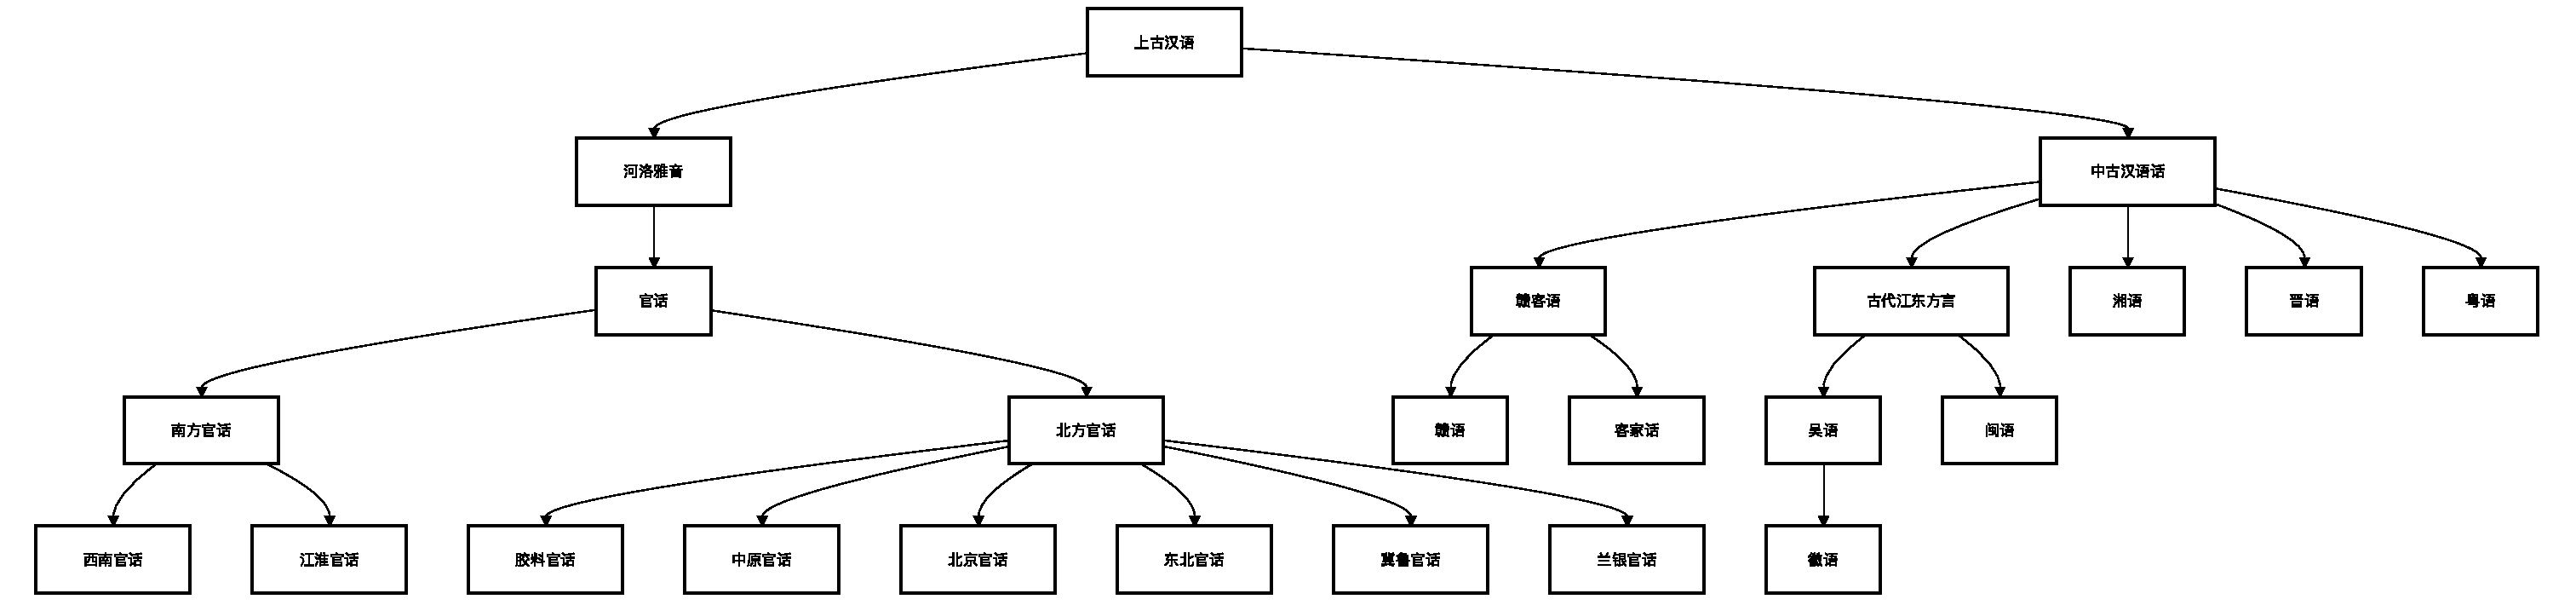
\includegraphics[width=\textwidth]{images/linguisitc_tree.drawio.pdf}
\end{figure}
由于各省之间存在大量的方言,并且现实中缺乏各方言在各省市中的人口分布数据,本文根据《中国语言地图集》选取各省的代表性语言作为其方言指标。值得注意的是部分省份由于内部存在大量完全分割的语言,例如江苏就包括吴语与江淮官话,本文选取流入人口较多的苏州、无锡一带的吴语作为其代表性语言;又例如山东省内部存在胶辽官话、冀鲁官话、中原官话,本文以济南市的冀鲁官话作为其代表性语言。本文的具体设置如表格\ref{tab:方言分布表}所示。
同时本文还将各省市的普通话普及率纳入模型,数据来源则参考了\textcite{YuWeiQiGuoMinPuTongHuaNengLiDeJiBenZhuangKuangYuFaZhanTaiShi2018},从CGSS中获取。




\begin{table}[!ht]
\centering
\caption{方言分布表}
\begin{tabularx}{\textwidth}{@{}ccXccX@{}}
\toprule
\textbf{代表性方言} & \textbf{数量} & \multicolumn{1}{c}{\textbf{省份}} & \textbf{代表性方言} &\textbf{数量}  & \multicolumn{1}{c}{\textbf{省份}}\\
\midrule
西南官话 & 6 & 湖北省、广西壮族自治区、重庆市、四川省、贵州省、云南省 &晋语 & 2 &山西省、内蒙古自治区\\
东北官话 & 3 &辽宁省、吉林省、黑龙江省 & 北京官话  &1 &北京市\\
吴语 & 3 &浙江省、上海市、江苏省& 赣语  &1 &江西省\\
中原官话 & 3 &河南省、陕西省、青海省 &胶辽官话  &1& 山东省\\
冀鲁官话 & 2 &天津市、河北省、山东省 &湘语  &1 &湖南省\\
闽语 & 2 &福建省、海南省 &粤语  &1& 广东省\\
兰银官话 & 2 &甘肃省、宁夏回族自治区 &其他  &2& 西藏自治区、新疆维吾尔自治区\\
\bottomrule
\end{tabularx}
\label{tab:方言分布表}
\end{table}


本文对于复合指标的获取如表格所示


\paragraph{同乡网络}

本文还是用了CMDS数据中的劳动力分布情况作为ABM中同乡网络,得到的数据分布如表格所示:




% ---------------------------------------- 估计结果 ----------------------------------------
\chapter{估计结果}

\section{基准回归与子样本分析} % (fold)


由LightGBM得到的训练结果数据如表格\ref{tab:机器学习插件训练结果}所示
\begin{table}[!ht]
\centering
\caption{结构参数结果}
\begin{tabularx}{\textwidth}{@{}cXXX@{}}
\toprule
\midrule
\bottomrule
\end{tabularx}
\label{tab:机器学习插件训练结果}
\end{table}




经过NFXP算法估计得到的参数值如下表格\ref{tab:结构参数的估计结果}所示。(附带标准误和显著性星号标记)
\begin{table}[!ht]
\centering
\caption{结构参数结果}
\begin{tabularx}{\textwidth}{@{}cXXX@{}}
\toprule
\midrule
\bottomrule
\end{tabularx}
\label{tab:结构参数的估计结果}
\end{table}

对这些数据的解读可以分为以下几点:
\begin{enumerate}
  \item 首先
  \item 然后
\end{enumerate}


\paragraph{有限混合的估计结果} 

优先混合类型的估计参数结果如下表格\ref{tab:有限混合参数的估计结果}所示。

本文报告了混合参数的标注误,但是没有其相关的显著性,这是因为...

\begin{table}[!ht]
\centering
\caption{有限混合参数的估计结果}
\begin{tabularx}{\textwidth}{@{}cXXX@{}}
\toprule
\midrule
\bottomrule
\end{tabularx}
\label{tab:有限混合参数的估计结果}
\end{table}


\paragraph{一些结论}

从模型的基础结果,我们可以回答以下问题:

- 户籍制度的影响途径是哪些

- 影响劳动力迁移最大的因素

- 家乡溢价的影响如何


\subsection{从回归结果解读迁移摩擦}
本文将得到的结果与先前学者的研究成果进行对比,其具体内容如表格\ref{tab:研究成果对比}所示。
\begin{table}[!ht]
\centering
\caption{研究成果对比}
\begin{tabularx}{\textwidth}{@{}cXXX@{}}
\toprule
\midrule
\bottomrule
\end{tabularx}
\label{tab:研究成果对比}
\end{table}



\section{模型的拟合检验} 


我们报告 Hit Rate、交叉熵和 Brier Score;并对关键分组的选择份额做误差分解,具体如下:
\begin{itemize}
  \item 对数似然 / 交叉熵(Cross-Entropy):更看重概率好坏;
  \item Brier Score(概率均方误差):直观;
  \item 分组命中:按省份/城市等级/年龄/教育分组的均值误差(ME/MAE/RMSE),保证结构性事实被复现。
\end{itemize}


还进行了
样本内拟合: 比较模型预测的迁移矩阵、各年龄段迁移率、返乡率等,与数据中的实际值。

样本外预测: 用2010-2018年的数据估计模型,然后用估计出的参数去预测2020、2022年的迁移模式,看预测得有多准。


\section{机制分解} % (fold)
\label{sec:机制分解}

机制分解 (Mechanism Decomposition):

目的: 量化不同“摩擦”的重要性。

实施:
用您估计出的完整模型进行一次基准模拟 (baseline simulation)。
反事实模拟1: 将$HukouPenalty$设为$0$,再模拟一次。
反事实模拟2: 将$\alpha_{home}$设为$0$,再模拟一次。
反事实模拟3: 将迁移成本$\kappa$中的距离项设为$0$,再模拟一次。

产出: 一张表格或一张图,清晰地展示“户籍制度”、“家乡情感”和“地理距离”分别解释了多大比例的人口流动不足或地区收入差距。


% ---------------------------------------- ABM模块 ----------------------------------------
\chapter{与宏观桥接} % (fold)
\label{sec:与宏观桥接}

本文使用ABM机制释放微观模型的宏观解释力,增强模型的现实意义。


\section{抽样映射与} % (fold)
\label{sub:抽样映射与}


在 ABM 初始化中,我们基于有限混合估计结果构造代理群体。具体而言,对每个代理$a$独立抽样类型$z_a\sim Categorical(\hat \pi_1,\dots,\hat \pi_M)$,并继承该类型的参数向量 $\theta_{z_a}$。因此代理的决策规则等价于在条件于 $(x_a,z_a)$ 下使用结构估计得到的 CCP。个体观测特征(如年龄、教育、家乡)则按基准期数据经验分布抽样生成。这样实现了从有限混合的微观估计到 ABM 个体代理的自然映射。




$𝑇_1$:完全理性(沿用你的 NFXP-Bellman 决策)。

$𝑇_2$:Quantal Response / 噪声理性:选择概率服从$\exp(utility/\lambda)$ ,$\lambda>0$表示误差分散度。

$𝑇_3$:前景理论型:已有的$U^{income}$继续保留;再允许损失厌恶参数、概率加权(可简化为 piecewise S 型)。

$T_4$:启发式/规则型:阈值规则(如“收入提高超过$\tau$且户籍惩罚低于$\kappa$就迁”),用于对比基准。





\section{外部性机制} % (fold)
\label{sec:外部性机制}

外部性机制(房价拥挤、同乡网络、就业拥挤):这是 ABM 的增量价值 —— 你在结构估计中无法自然引入的宏观反馈,在 ABM 世界里能释放出来。

拥挤/房价/通勤成本反馈:城市 j 的净吸引力随流入量上升而递减(可把你的“目的地舒适度” $y_{sj}(K_t)$ 动态化)。

社交网络/同乡效应:迁移成本$\kappa_{it}$随同乡存量下降(信息/中介降低成本),或加入“推荐效应”。

用工需求/匹配面:简单的 DMP/招聘配额或“岗位随机分配”模块,让工资项 $w_{itj}$ 也随时点与总量反馈。



\section{模型校准} % (fold)
\label{sub:模型校准}





传统模拟校准使用Simulated Method of Moments(SMM/Indirect Inference):选一组目标矩(如省际净流入率、返乡率、跨省占比、年龄结构、目的地集中度 Herfindahl、同乡聚集度),最小化“数据矩 vs 模拟矩”的距离。

本文尝试使用ABM模拟一个可交互的环境进行SMM。
使用ABM对劳动力流动进行研究并不是一个新鲜的事情,例如\textcite{fuAgentBasedModelingChinas2018,klabundeDecisionmakingAgentbasedModels2016}。

使用SMM校准ABM是主流路线(\textcite{plattComparisonEconomicAgentbased2020}),进来也不乏对于使用ABM进行校准的探索,例如\textcite{rahmandadUsingMethodSimulated2015}和\textcite{pietzschMetamodelsEvaluatingCalibrating2020}。

ABM 校准本质上就是在“模拟器”上做 SMM/II。区别只在于 ABM 的状态演化带外部性,模拟更“厚重”。

工作流:
\begin{enumerate}
\item 选目标矩(少而精,10–30 个);
\item 给每个矩设权重(或用协方差矩阵做 GMM 权重);
\item 用全局搜索 + 局部优化(如 differential evolution → BFGS)找参数;
\item 做交叉年份验证与敏感性(目标矩替换/权重扰动)。
\end{enumerate}


此处给出的结果不会过多强调显著性,因为 ABM 校准不是通过似然估计,而是通过 SMM 或最小距离匹配出来的“标定值”。

文献习惯报告目标矩的拟合优度(例如真实值 vs 模拟均值 vs 模拟区间),而不是给“显著性星号”。



\section{ABM模型的检验} % (fold)
\label{sub:abm模型的检验}


基准验证与宏观涌现分析:

实施: 运行校准好的ABM模型,观察是否能自发地“涌现”出一些宏观层面的模式,例如:
\begin{itemize}
  \item 城市规模的齐普夫定律 (Zipf's Law)。
  \item “胡焕庸线”两侧的人口密度差异。
  \item “孔雀东南飞”后又出现的回流潮。
\end{itemize}




产出: 

将模拟出的宏观模式与真实数据进行对比,展示您模型的宏观现实性。




\section{反事实参数估计}
移动户籍障碍,查看其他变量的变化情况


本文的做法是在已有 ABM+SMM / data-driven ABM 的框架下,把严谨估计的 DDCM 参数转为 ABM 校准并用于政策反事实。

产出不再是简单的静态比较,而是动态演化图。例如:一张线图,展示在“取消户籍”政策冲击后,北京、上海的人口如何在未来20年内先上升后因拥挤效应而趋于平稳,而成都、武汉的人口则持续上升。或者一张地图面板,展示全国人口密度在不同政策情景下随时间演变的动态视频或系列图片。



政策实验:分阶段放宽户籍、发放落户补贴、公共服务均等化、“二线城市吸引力提升”、“首次迁移 vs 返乡补贴”、“户籍门槛分层”等高含金量的政策实验。

反事实:取消家乡溢价/加大家乡溢价、提升二线城市宜居度、限制超大城市增量指标等。

稳健性:比较$T_1\sim T_4$组合与现实事实的匹配度,论证“有限理性/网络效应”的必要性。



\paragraph{Step 0:基线对齐}

用 2010–2020 校准好的参数运行 ABM,确保关键矩被复现(§3 的目标矩)。

固定随机种子,重复 
R=20 次,报告均值与置信区间。

\paragraph{Step 1:定义清晰的政策杠杆(只改一两处)}

常见而有意义的杠杆与其对应模型变量:

落户门槛/指标:降低 
HukouPenalty 或提高“积分落户名额”。
迁移补贴/交通补助:降低 
的固定项或与距离相关项。
公共服务均等化:提高低线城市的 ) 子项(医疗/教育)。
住房政策:控制高线城市的房租弹性(通过  或供给弹性)。
信息/中介服务:增大同乡效应 (降低首次迁移门槛)。

\paragraph{Step 2:设定“路径”而非“静态点”}

例如 2014–2018 分阶段放松落户:
或者只在 若干试点城市实施(空间异质性)。

\paragraph{Step 3:结果面板(必报 + 选报)}

人口/流向:各城市净流入率、省际/省内迁移占比、返乡率。
劳动力结构:年龄×教育分布、技能错配率。
福利/效用:个体期望折现效用的变化(或等价收入);
市场压力:房租指数、拥挤度指标、岗位空缺率。
空间均衡:基尼/泰尔指数衡量地区收入与人口集中度。
报告 短期(1–3 年)/中期(5 年)/长期(10 年) 路径。

\paragraph{Step 4:稳健性与权衡}

Pareto 前沿:横轴“地区均衡(如人口集中度↓)”,纵轴“总福利/产出”;展示不同政策强度/配比的前沿。
敏感性:对(外部性强度)、岗位容量弹性、同乡网络初始值做 $\pm 25\%$ 变动。

\paragraph{三个“高含金量”的政策场景}

“二线吸引力提升 + 落户同步放松”:

提高二线城市  若干子项(公共服务)+ 降低其 HukouPenalty。
看点:是否能从超大城市“吸”出新增人口而不牺牲总产出;流向是否更均衡。

“首次迁移补贴 vs 返乡补贴”的对照:

设计同等财政成本:要么给首次跨省迁移者发补贴(降 
κ 固定项),要么给返乡者发补贴。
看点:哪种更能提升长期人岗匹配/地区均衡;是否出现“补贴循环”(来回搬)。

“户籍门槛分层 + 名额随机/积分排序”

在模型内实现“名额”制度:超过配额者增加额外惩罚。
看点:不同分配机制(随机 vs 积分)对选择边际人群与社会福利的差异。







% ---------------------------------------- 结论 ----------------------------------------
\chapter{结论与展望}

结构识别+ML稳健性+ABM宏观解释


当然以城乡二元对立为代表的思想在我国依旧有非常重要的应用 因为我国依旧有大量依附于城乡关系的社会体系、福利体系等种种重要的制度
甚至在研究二元对立话题中依旧可以引入例如Rosen Roback这样的经典模型
例如 
\textcite{GuoDongMeiChengXiangRongHeDeShouRuHeFuLiXiaoYingYanJiuJiYuYaoSuPeiZhiDeShiJiao2023}指出城乡融合的收入和福利效应研究——基于要素配置的视角
但对于在破除劳动力迁移摩擦、开放劳动力要素自由流动的当下
抛开这种二元对立的思想是越来越重要的
这也自然而然地引出了空间均衡与最有选址两种思路



由于普遍偏好事少离家近的特征,政策可以针对性地对周边省份进行补贴
相反 对于十分遥远地区的人力资源 即使补贴了显性的迁移成本 也存在较长的文化、心里距离 所以在边际上可能并不值得投入



本文可以改进的地方:

添加约束

添加宏观变量

使模型作为微观基础从而宏观化
\textit{近年来,一些研究将上述两种基础模型结合起来,在空间均衡模型中加入了微观层面的动态迁移决策特征。这些动态一般均衡迁移模型明确考虑了空间工资差异的来源及其对净迁移和总迁移的影响,并允许存在不同类型的空间障碍,如劳动力重新配置摩擦和信息摩擦。这类模型特别关注迁移如何作为调节各地劳动力市场长期均衡的机制。例如,Coen-Pirani(2010)开发了一个动态一般均衡模型,强调了个体迁移决策中的不可观测异质性。该模型刻画了总迁移流动和净迁移流动的共同模式,其中前者由个体匹配的偶然冲击驱动,后者由持续的生产率冲击驱动。工人会迁移到正受到生产率冲击的地区,并在迁移后发现其偶然匹配的质量。新迁移的工人比长期居住者更可能继续迁移,因为后者选择留在某地是由于他们已经获得了相对较好的匹配。该校准模型可以解释为何人口流入较多的地区往往也伴随着较多的流出,这一现象在仅研究净流入的模型中无法得到解释。结合偶然匹配效应的空间均衡模型还能够解释新迁入工人与迁出工人在年龄、教育和行业等方面的相似性,这些特征无法仅通过个体位置选择模型或仅基于可观测工人异质性或地点特定冲击的模型来解释。}

从而引入其他变量

以家庭为基本单位


% ---------------------------------------- 附录 ----------------------------------------
\newpage
\appendix

\chapter{详细的语言谱系树}

A TREE

======

      ||
      
      ||
      
      ||

\newpage
%\bibliography{Papers}
%\bibliographystyle{gbt7714-plain}
%\bibliographystyle{gbt7714-author-year}
\printbibliography[heading=bibliography,title=参考文献]
\end{document}
